\part{概率论}
\section{概率事件和概率}
\subsection{事件、关系与运算}
事件的关系有
\begin{enumerate}[(1)]
    \item 包含关系:一个事件$A$包含另一个事件$B$记作:$B\subset A$。这时只要事件$B$发生,那么事件$A$也一定发生;
    \item 等价关系:两个事件对应的子集完全相等,记作$A=B$;
    \item 对立关系:两个事件只能有一个发生,并且必然有一个发生,则它们是对立关系;
    \item 互斥关系:两个事件只能有一个发生,但并不必然有一个发生。这时也称两个事件之间是互不相容的;
    \item 如果两个事件同时发生的概率等于它们各自发生的概率的乘积,那么就称这两个事件是相互独立的。
\end{enumerate}

事件的运算有三种
\begin{enumerate}[(1)]
    \item 事件$A\cup B$:是事件$A$和事件$B$的和事件(并事件),指的是事件“事件$A$发生或者事件$B$发生”;
    \item 事件$AB$或者$A\cap B$:是事件$A$和事件$B$的积事件(交事件),指的是事件“事件$A$发生且事件$B$发生”;
    \item 事件$A-B$:是事件$A$和事件$B$的差事件,指的是事件“事件$A$发生且事件$B$不发生”。
\end{enumerate}

对于事件运算和事件关系之间的联系有:
\begin{enumerate}[(1)]
    \item $AB$互斥或不相等,则有$AB=\emptyset$;
    \item $A,B$互为对立事件,则有$AB=\emptyset, A\cup B=\Omega$(全集);
    \item $A-B = A\overline{B} = A-AB$;
    \item $A\overline{A}=\emptyset$
\end{enumerate}

事件的运算规律:
\begin{enumerate}[(1)]
    \item 交换律:$A\cup B = B\cup A, AB = BA$;
    \item 结合律:$A\cup(B\cup C) = (A\cup B)\cup C,A(BC) = (AB)C$;
    \item 分配律:$A(B\cup C) = AB\cup AC, A\cup(BC) = (A\cup B)(A\cup C)$;
    \item 对偶律:$\overline{A\cup B} = \overline{A}\cap \overline{B}, \overline{AB}=\overline{A}\cup\overline{B},\overline{A-B}=\overline{A\overline{B}}=\overline{A}\cup B$
    \item $A\supset B \iff \overline{A}\subset \overline{B}$
\end{enumerate}

\begin{example}
    设$A\cup B = \overline{A}\cup\overline{B}$,则有
    \begin{tasks}[label=(\Alph*),label-width = 2em](2)
        \task $A-B=\emptyset$
        \task $AB=\emptyset$
        \task $AB\cup \overline{A}\overline{B}=\Omega$
        \task $A\cup \overline{B}=\Omega$
    \end{tasks}
\end{example}

\begin{solution}
    \begin{align*}
        A(A\cup B)                      & = A \cup AB = A                                       \\
        A(\overline{A}\cup\overline{B}) & = \emptyset \cup A\overline{B} = A\overline{B} = A-AB
    \end{align*}
    因此$A=A - AB$,显然$AB=\emptyset$,选(B)
\end{solution}

\subsection{概率统计}
概率相关的性质
\begin{enumerate}[(1)]
    \item $P(\emptyset) = 0$;
    \item 可加性$\displaystyle P(\bigcup_{i=1}^n A_i) = \sum_{i=1}^n P(A_i)$;
    \item $P(\overline{A}) = 1 - P(A)$;
    \item 若$A\subset B$,则$P(A)\leq P(B)$;
    \item $0\leq P(A)\leq 1$
\end{enumerate}
\textcolor{red}{在计算概率的时候,永远无法从概率推出事件的关系}。


\subsection{独立事件}
在概率论里,说两个事件是独立的,直觉上是指一次实验中一事件的发生不会影响到另一事件发生的概率。
\begin{definition}
    两个事件$A$和$B$是独立的当且仅当\[ P(AB) = P(A)P(B) \]
\end{definition}
这里一定要注意的是:独立、互斥是两码事。(不可能事件与任何事件独立,互斥;$P(A)=0$的$A$事件与任何事件独立)

这里有一个经常出的知识点:三个事件相互独立
\[
    \begin{cases}
        P(ABC)=P(A)P(B)P(C) \\
        P(AB)=P(A)P(B)      \\
        P(AC)=P(A)P(C)      \\
        P(BC)=P(B)P(C)
    \end{cases}
\]
而两两独立指的是:两个事件之间是否独立,即$P(AB)=P(A)P(B)$。

那么显然,在一些事件中,相互独立则是有两两独立的;但两两独立,不能得出相互独立。

\begin{property}
    假设$A,B$独立,则下面这些也是独立的
    \begin{enumerate}[(1)]
        \item $A,\overline{B}$;
        \item $\overline{A},B$;
        \item $\overline{A},\overline{B}$。
    \end{enumerate}
\end{property}
换句话说“补”操作不影响独立性质。

\begin{property}
    当$0<P(B)<1$时,$A,B$独立等价于$P(A \mid B) = P(A \mid \overline{B})$
    亦等价于$P(A\mid B) = P(A)$
\end{property}

\subsubsection{条件概率}
.
\begin{definition}
    条件概率就是事件$A$在事件$B$发生的条件下发生的概率。条件概率记为为$P(A\mid B)$。
    \[ P(B)>0\qquad P(A\mid B) = \frac{P(AB)}{P(B)} \]
\end{definition}

条件概率其实就是缩减样本空间,那么可以根据$P(A)=1-P(\overline{A})$,得出
\begin{eqnarray}
    P(A\mid B) = 1 - P(\overline{A}\mid B)
\end{eqnarray}

与独立事件相联系,就有下面这个公式:
\begin{equation}
    A,B\text{独立} \iff P(A\mid B) = P(A\mid \overline{B}) = P(A)
\end{equation}
也就是$B$是否发生,都不影响$A$发生,也就是$A,B$独立。

\subsection{概率五大公式}
\begin{enumerate}[(1)]
    \item 加法公式:
          \begin{align*}
              P(A\cup B)       & = P(A)+P(B)-P(AB)                         \\
              P(A\cup B\cup C) & = P(A)+P(B)+P(C)-P(AB)-P(BC)-P(CA)+P(ABC)
          \end{align*}
    \item 减法公式:$ P(A-B)=P(A)-P(AB) $
    \item 乘法公式:$ P(AB) = P(A)P(B\mid A),\qquad P(A)>0  $
    \item 全概率公式:完备事件组$\{A_1,A_2,\cdots,A_n \}$,即$\bigcup_{i=1}^n A_i = \Omega, A_iA_j = \emptyset, P(A_i)>0$,则对于任意一个事件$B$,有
          \[ P(B) = \sum_i^n P(BA_i) = \sum_i^n P(B\mid A_i)P(A_i) \]
    \item 贝叶斯公式:完备事件组$\{A_1,A_2,\cdots,A_n \}$,则任意一个事件$A_j$有
          \[ P(A_i\mid B) = \frac{P(A_i)P(B\mid A_i)}{\sum_{j=1}^n P(B\mid A_j)P(A_j)} \]
          其中分母为全概率公式。简单形式为随机事件$A,B$且$P(B)>0$,则有
          \[ P(A\mid B) = \frac{P(A)P(B \mid A)}{P(B)} \]
\end{enumerate}

\subsection{古典概型、伯努利概型}
当样本空间\textcolor{red}{有限},试验中每个基本事件发生\textcolor{red}{的可能性相同}的时候,称为\textcolor{red}{\textbf{\textsf{古典概型}}}。
\begin{example}
    设一个三位数,其中三个数字两两不同的概率?
\end{example}
\begin{solution}
    第一位数字$1,2,\cdots,9$,第二位第三位数字是$0,1,\cdots,9$则一共有$900$种可能,
    其中两两不同一共有$C_9^1\cdot C_9^1\cdot C_8^1=648$,故概率为
    \[ P=\frac{648}{900} = 0.72 \]
\end{solution}
\begin{example}
    $6$个产品种有两个次品,先每次一个地逐个随机抽取,求
    \begin{enumerate}[(I)]
        \item 恰好抽三次就确定$2$个次品的概率$P(A)$;
        \item 不超过三次就确定$2$个次品的概率$P(B)$。
    \end{enumerate}
\end{example}
\begin{solution}
    \begin{enumerate}[(1)]
        \item 恰好抽三次就确定$2$个次品,说明前两次抽取只有一个次品,第三次抽出次品,即从$6$个产品中任取$2$个,其中一个次品为第三次抽取,另一个次品为前两次抽取:
              \[ P(A) = \frac{C_2^1C_1^1}{C_6^2} = \frac{2}{15} \]
        \item 不超过三次确定两个次品,则要抽两次或三次,即$6$个产品任取$2$个,其中抽到两个次品放在前三次抽取:
              \[ P(B) = \frac{C_3^2}{C_6^2} = \frac{1}{10} \]
    \end{enumerate}
\end{solution}

\textcolor{red}{\textbf{\textsf{伯努利试验}}}指的是单次事件,而这次事件的结果是两个可能性结果中的一个。
\begin{example}
    某选手打靶命中率为$0.5$,连射三次后检查靶后发现已经命中,求他再第一次射击时就已命中的概率。
\end{example}
\begin{solution}
    设$A$为三次射击至少命中一次,$B$为第一次射击命中,显然$B\subset A$
    则有
    \[ P(B|A) = \frac{P(BA)}{P(A)} = \frac{P(B)}{P(A)} = \frac{P(B)}{1-P(\overline{A})} = \frac{0.5}{1-0.5^3} = \frac{4}{7} \]
\end{solution}
\section{随机变量和分布}
给定样本空间$(S,\mathbb{F})$,如果其上的实值函数 $X:S\to \mathbb {R}$是$\mathbb{F}$(实值)可测函数,则称
$X$为\textcolor{red}{\textbf{\textsf{随机变量}}}。

如果随机变量$X$的曲子时有限的或则是可数无穷尽的值,
\[ X=\{ x_1,x_2,\cdots, \} \]
则称$X$为\textcolor{red}{离散}随机变量。

如果$X$由全部实数或者由一部分区间组成,
\[ X=\{ x\mid a\leq x\leq b \}, -\infty <a<b< +\infty\]
则称$X$为\textcolor{red}{连续}随机变量.


\begin{example}
    从$1,2,3,4$中任取$2$个数,其中小的数记为$X$,求$X$的分布律
\end{example}
\begin{solution}
    $X$的取值范围为${1,2,3}$,则有
    \begin{align*}
        P(X=1) & = \frac{C_3^1}{C_4^2} = \frac{1}{2} \\
        P(X=2) & = \frac{C_2^1}{C_4^2} = \frac{1}{3} \\
        P(X=3) & = \frac{C_1^1}{C_4^2} = \frac{1}{6}
    \end{align*}
    因此$X$的分辨律为
    \begin{center}
        \begin{tabular}{c|ccc}
            $X$ & $1$           & $2$           & $3$           \\ \hline
            $P$ & $\frac{1}{2}$ & $\frac{1}{3}$ & $\frac{1}{6}$
        \end{tabular}
    \end{center}
\end{solution}

\begin{definition}
    对于随机变量$X$,$X\leq x$的概率记为随机变量$X$的分布函数$F(x)$,即
    \[ F(x) = P\{X \leq x\},\qquad -\infty < x < +\infty \]
\end{definition}
显然对于分布函数,有如下性质
\begin{enumerate}[(1)]
    \item $ 0\leq F(x) \leq 1 $;
    \item $ F(x) $单调非降;
    \item $ \lim_{x\to -\infty} F(x) = 0, \lim_{x\to +\infty}F(x) = 1 $;
    \item $F(x)$是右连续函数,即$F(x^+) = F(x)$;
    \item $\forall x_1<x_2, P\{x_1<X\leq x_2\} = F(x_2) - F(x_1)$;
    \item $\forall x, P\{X=x\} = F(x)-F(x^-) = F(x) - \lim_{x\to x^-} F(x)$
\end{enumerate}
若一个函数满足性质(1)到(4),则这个函数是分布函数。

\begin{example}
    若
    \begin{tabular}{c|ccc}
        $X$ & $1$           & $2$           & $3$           \\ \hline
        $P$ & $\frac{1}{3}$ & $\frac{1}{2}$ & $\frac{1}{6}$
    \end{tabular}
    求$X$的分布函数$F(x)$。
\end{example}
\begin{solution}
    由于分布函数是右连续,故区间是左闭右开,所以将$(-\infty,+\infty)$分为$4$个部分,
    \[
        F(x) = P\{ X\leq x \}
        =
        \begin{dcases}
            0,           & x< 1,        \\
            \frac{1}{3}, & 1\leq x < 2, \\
            \frac{5}{6}, & 2\leq x < 3, \\
            1 ,          & 3\leq x
        \end{dcases}
    \]
\end{solution}

\begin{definition}
    对于随机变量$X$,设它的分布函数为$F(x)$,如果存在函数$f(x)$,满足:
    \[ F(x) = \int_{-\infty}^x f(t)\dd{t}, \qquad \forall x \in (-\infty,+\infty) \]
    那么X 是一个\textcolor{red}{连续型}随机变量,$f(x)$是量$X$的概率密度函数。
\end{definition}
显然连续型随机变量$X$的分布函数$F(x)$是连续函数。

概率密度函数$f(x)$有如下性质:
\begin{enumerate}[(1)]
    \item $f(x)\geq 0$;
    \item $\displaystyle \int_{-\infty}^{+\infty} f(x)\dd{x} = 1$;
    \item $\displaystyle P\{ x_1< X \leq x_2 \} = \int_{x_1}^{x_2} f(t)\dd{t} = F(x_2)-F(x_1)$;
    \item 如果$f(x)$在$x$点上连续,那么$F(x)$可导,并且有$F'(x)=f(x)$
\end{enumerate}

\subsection{常见分布}
\subsubsection{二项分布}
$n$次成功率为$p$的伯努利试验的成功次数的分布,称为二项分布,记为$X\sim B(n,p)$。
且有
\begin{align}
    P\{ X=k \} & = C_n^k p^k(1-p)^{n-k}, k\in\{0,1,2,\cdots,n\} \label{eq:二项分布律} \\
    E(X)       & = np \label{eq:二项分布期望}                                         \\
    D(X)       & = np(1-p) \label{eq:二项分布方差}
\end{align}

\subsubsection{几何分布}
在伯努利试验中,得到一次成功所需要的试验次数$X$,称为几何分布,记为$X\sim G(p)$。且有
\begin{align}
    P\{X=k\} & = (1-p)^{k-1}p, k\in\{0,1,2,3,\cdots \} \label{eq:几何分布律} \\
    E(X)     & = \frac{1}{p} \label{eq:几何分布期望}                         \\
    D(X)     & = \frac{1-p}{p^2} \label{eq:几何分布方差}
\end{align}

\subsubsection{超几何分布}
有$N$个样本,其中$K$个是不及格的。超几何分布描述了在该$N$个样本中抽出$n$个,其中$k$个是不及格的几率:
\[ P\{ X=k \} = \frac{C_K^k C_{N-K}^{n-k}}{C_N^n} \]

上式可如此理解:$C_N^n$表示所有在$N$个样本中抽取$n$个的方法数目,$C_K^k$表示在$K$个样本中,抽取$k$个的方法数目,剩下的$N-k$个都是及格的,
剩下的抽法就有$C_{N-K}^{n-k}$种。

\subsubsection{泊松分布}
泊松分布适合于描述单位时间内随机事件发生的次数的概率分布。若$X$付出参数为$\lambda$的泊松分布,记为$X\sim P(\lambda)$。
泊松分布的参数$\lambda>0$是单位时间(或单位面积)内随机事件的平均发生次数。且有
\begin{align}
    P\{ X=k \} & = \frac{\lambda^k}{k!}\mathrm{e}^{-\lambda}, k\in\{0,1,2,3,\cdots\} \label{eq:泊松分布分布律} \\
    E(X)=D(X)  & =\lambda \label{eq:泊松分布期望方差}
\end{align}

两个独立且服从泊松分布的随机变量$X,Y$,其和仍然满足泊松分布,即
\[ X\sim P(\lambda_1), Y\sim P(\lambda_2) \implies X+Y \sim P(\lambda_1+\lambda_2) \]

泊松分布与泰勒展开:
\[
    \sum_{k=0}^\infty \frac{\lambda^k}{k!}\mathrm{e}^{-\lambda} = 1,
    \qquad
    \sum_{k=0}^\infty \frac{\lambda^k}{k!} = \mathrm{e}^\lambda
\]

\subsubsection{均匀分布}
.
\begin{marginfigure}
    \centering
    \begin{tikzpicture}
        \begin{axis}[
                axis lines=middle,
                ymin=0,ymax=2,
                xmin=0,xmax=3,
                xlabel=$x$,
                ylabel=$y$,
                scale only axis,
                xtick={1,2},
                xticklabels={$a$,$b$},
                ytick={1},
                yticklabels={$\frac{1}{b-a}$},
                yticklabel style={anchor=west},
                width=0.9\textwidth
            ]
            \draw[color=magenta] (axis cs:1,1) -- (axis cs:2,1);
            \addplot[color=magenta,only marks,style={mark=*,fill=white}] coordinates {(1,0)} ;
            \addplot[color=magenta,only marks,style={mark=*}] coordinates {(1,1)} ;
            \draw[color=magenta!50!white,dashed] (axis cs:1,0) -- (axis cs:1,1);
            \addplot[color=magenta,only marks,style={mark=*,fill=white}] coordinates {(2,0)} ;
            \addplot[color=magenta,only marks,style={mark=*}] coordinates {(2,1)} ;
            \draw[color=magenta!50!white,dashed] (axis cs:2,0) -- (axis cs:2,1);
        \end{axis}
    \end{tikzpicture}
    \caption{均匀分布概率密度函数}
\end{marginfigure}
\begin{marginfigure}
    \centering
    \begin{tikzpicture}
        \begin{axis}[
                axis lines=middle,
                ymin=0,ymax=1.5,
                xmin=0,xmax=4,
                xlabel=$x$,
                ylabel=$y$,
                scale only axis,
                xtick={1,3},
                xticklabels={$a$,$b$},
                ytick={1},
                yticklabels={1},
                yticklabel style={anchor=west},
                width=0.9\textwidth
            ]
            \draw[color=magenta] (axis cs:0,0) -- (axis cs:1,0) -- (axis cs:3,1) -- (axis cs:4,1);
            \draw[color=magenta!50!white,dashed] (axis cs:0,1) -- (axis cs:3,1);
        \end{axis}
    \end{tikzpicture}
    \caption{均匀分布累积分布函数}
\end{marginfigure}

\begin{definition}
    一个均匀分布在区间$[a,b]$上的连续型随机变量$X$,称为$X$服从均匀分布,记为$X\sim U[a,b]$,且
    \begin{align*}
        f(x) & =
        \begin{dcases}
            \frac{1}{b-a} & x \in [a,b]                     \\
            0             & x \in(-\infty,a)\cup(b,+\infty)
        \end{dcases} \\
        F(x) & =
        \begin{dcases}
            0               & x<a          \\
            \frac{x-a}{b-a} & a\leq x < b, \\
            1               & b\leq x
        \end{dcases}
    \end{align*}
\end{definition}

对于均匀分布的概率求法,一般在概率密度函数图上,直接利用几何关系求矩形面积。

\subsubsection{指数分布}
指数分布是一种连续概率分布。指数分布可以用来表示独立随机事件发生的时间间隔,例如放射性核素的半衰期。
\begin{marginfigure}
    \centering
    \begin{tikzpicture}
        \begin{axis}[
                ticks=none,
                axis lines=middle,
                ymin=0,ymax=1.5,
                xmin=-1,xmax=4,
                xlabel=$x$,
                ylabel=$y$,
                scale only axis,
                width=0.9\textwidth
            ]
            \draw[color=magenta,thick] (axis cs:-1,0) -- (axis cs: 0,0);
            \addplot[color=magenta,only marks,style={mark=*}] coordinates {(0,0)} ;
            \addplot[color=magenta,only marks,style={mark=*,fill=white}] coordinates {(0,1)} ;
            \addplot[color=magenta, domain=0:4] {exp(-x)};
        \end{axis}
    \end{tikzpicture}
    \caption{指数分布概率密度函数}
\end{marginfigure}
\begin{definition}
    如果一个随机变量$X$满足
    \[
        f(x) =
        \begin{cases}
            \lambda \mathrm{e}^{-\lambda x}, & x>0,    \\
            0,                               & x\leq 0
        \end{cases}
        ,\qquad \lambda > 0
    \],则称$X$服从指数分布,记作$X\sim E(\lambda)$
\end{definition}
若$X\sim E(\lambda)$,则有如下性质
\begin{enumerate}[(1)]
    \item $\displaystyle P\{ X > t \} = \int_t^{+\infty} \lambda \mathrm{e}^{-\lambda x}\dd{x} = \mathrm{e}^{-\lambda t}, (t>0)$;
    \item $\displaystyle P\{ X > t \} = 1, (t\leq 0)$;
    \item $P\{ X > t+s \mid X>s \} = \dfrac{P\{ X>t+s \}}{P\{X > s\}} = \mathrm{e}^{-\lambda t} = P\{ X>t \}, (s,t>0)$(无记忆性);
    \item $\displaystyle \int_0^{+\infty} x^n \mathrm{e}^{-x} \dd{x} = \Gamma(n+1) = n! $
\end{enumerate}

其中(2)类比放射性核素衰变,在已经衰变$s$秒后,此时再衰变$t$秒,与直接衰变$t$秒是等价的,即放射性核素衰变不会被之前的衰变所影响。

\subsubsection{正态分布}
.
\begin{marginfigure}
    \centering
    \begin{tikzpicture}
        \begin{axis}[
                ticks=none,
                axis lines=middle,
                ymin=0,ymax=1,
                xmin=-2,xmax=2,
                xlabel=$x$,
                ylabel=$y$,
                scale only axis,
                width=0.9\textwidth
            ]
            \addplot[color=magenta, domain=-2:2,smooth] {0.8*exp(-2*x^2)};
        \end{axis}
    \end{tikzpicture}
    \caption{正态分布概率密度函数}
\end{marginfigure}
\begin{definition}
    若随机变量$X$服从一个位置参数为$\mu$,尺度参数为$\sigma$的正态分布,记为$X\sim N(\mu,\sigma^2)$,其概率密度为
    \[ f(x) = \frac{1}{\sigma\sqrt{2\pi}}\mathrm{e}^{-\frac{(x-\mu)^2}{2\sigma^2}} \]
    特别的,称$X\sim N(0,1)$为$X$服从标准正态分布,此时密度函数记为$\varphi(x)$,
    \[ \varphi(x)=\frac{1}{\sqrt{2\pi}}\mathrm{e}^{-\frac{x^2}{2}} \]
    其标准正态分布函数记为
    \[ \Phi(x) = \int_{-\infty}^x \varphi(x)\dd{x} \]
\end{definition}
任何正态分布,可通过变换$\frac{x-\mu}{\sigma}$后变为标准正态分布,这个过程称为标准化。

正态分布具有如下性质
\begin{enumerate}[(1)]
    \item 概率密度函数关于$\mu$对称;
    \item $\Phi(-x)=1-\Phi(x),\ \Phi(x)=1-\Phi(-x),\ \Phi(0)=\frac{1}{2}$;
    \item $X\sim N(0,1), a>0, P\{\abs{X}\leq a\} = 2\Phi(a)-1$
\end{enumerate}
计算一维正态分布相关的题目时,常常需要查表、标准化、利用对称性来求解。

\subsection{随机变量函数的分布}
若$X$是随机变量,则$Y=g(X)$也是随机变量。

如果$X$是离散型随机变量,则$Y$的分布律为
\[
    \begin{array}{c|ccccc}
        X & x_1    & x_2    & \cdots & x_n    & \cdots \\ \hline
        P & p_1    & p_2    & \cdots & p_n    & \cdots \\ \hline
        Y & g(x_1) & g(x_2) & \cdots & g(x_n) & \cdots
    \end{array}
\]
然后对上面的分布律\textcolor{red}{整理},相等的$Y$概率相加,从小到大排列。

如果$X$是连续型随机变量,则$Y=g(X)$\textcolor{red}{一般}也是连续型随机变量。求$f_Y(y)$一般利用定义法来做:
\[ F_Y(y) = P\{ Y\leq y \} = P\{ g(X)\leq y \} = P\left\{X \leq g^{-1}(y) \right\} = \int_{-\infty}^{g^{-1}(y)} f_X(x)\dd{x} = F_X(g^{-1}(y)) \]

\begin{example}
    \[
        X \sim f(x) =
        \begin{dcases}
            \frac{1}{3\sqrt[3]{x^2}}, & 1\leq x \leq 8, \\
            0,                        & \text{其它}
        \end{dcases}
    \]
    其中$F(x)$是$X$的分布函数,求随机变量$Y=F(X)$的分布函数$F_Y(y)$
\end{example}
\begin{solution}
    \[
        F(x) = \int_{-\infty}^x f(t)\dd{t} =
        \begin{cases}
            0 ,              & x<1,         \\
            \sqrt[3]{x} - 1, & 1\leq x < 8, \\
            1,               & 8\leq x.
        \end{cases}
    \]
    因此$Y=F(X)$的值域为$[0,1]$,因此

    当$y<0$时,$F_Y(y) = P\{Y\leq y\} = 0$;

    当$0\leq y \leq 1$时,
    \begin{align*}
        F_Y(y) & = P\{Y\leq y\} = P\{ F(X)\leq y \} = P\left\{ \sqrt[3]{X} - 1 \leq y \right\} = P\left\{ X \leq (y+1)^3 \right\} \\
               & = F\left((y+1)^3\right) = y
    \end{align*}

    当$y>1$时,$F_Y(y) = P\{Y\leq y\} = 1$

    综上可得,
    \[
        F_Y(y) =
        \begin{cases}
            0, & y<0,            \\
            y, & 0\leq y \leq 1, \\
            1, & 1<y.
        \end{cases}
    \]
\end{solution}
注意,有些问题中端点需要特别考虑,这牵扯到端点连续的问题。

这道题可以知道,若$Y=F_X(X)$,且$F_X^{-1}$存在,则有$Y\sim U[0,1]$,这是因为
\[
    F_Y(y) = P\{Y\leq y\} = P\{ F_X(X) \leq y \} = P\left\{ X \leq F_X^{-1}(y) \right\} = F_X\left(F_X^{-1}(y)\right) = y
\]

\begin{example}
    \[
        X\sim f(x) =
        \begin{cases}
            \abs{x}, & \abs{x}\leq 1, \\
            0,       & \text{其它}.
        \end{cases}
    \]
    求$Y=X^2+1$的概率密度函数$f_Y(y)$
\end{example}
\begin{solution}
    \[ F_Y(y) = P\{ Y\leq y \} = P\left\{ X^2+1 \leq y \right\} = P\left\{ X^2 \leq y-1 \right\} \]

    当$y<1$时,显然$F_Y(y) = P\left\{ X^2 \leq y-1 \right\} = 0$

    当$1\leq y\leq 2$时$\displaystyle F_Y(y) = P\left\{ -\sqrt{y-1} \leq X \leq \sqrt{y-1} \right\} = \int_{-\sqrt{y-1}}^{\sqrt{y-1}} \abs{x}\dd{x} =y-1$

    当$2<y$时,显然$F_Y(y) = P\left\{ X^2 \leq y-1 \right\} = 1$

    所以有
    \[
        f_Y(y) = F_Y'(y) =
        \begin{cases}
            1, & 1\leq y \leq 2 \\
            0, & \text{其它}
        \end{cases}
    \]
\end{solution}

\begin{example}
    若$ X\sim N(0,1), Y=\max\{X,2\} $,则$F_Y(y)$
    \begin{tasks}[label=(\Alph*),label-width = 2em](2)
        \task 是连续函数
        \task 恰好有一个间断点
        \task 至少有两个间断点
        \task 是阶梯函数
    \end{tasks}
\end{example}
\begin{solution}
    \[ F_Y(y) = P\{ Y\leq y \} = P\{ \max\{X,2\}\leq y \} \]

    所以当$y<2$时,$F_Y(y)=0$

    当$y\geq 2$时,$F_Y(y) = P\{ \max\{X,2\}\leq y \} = P\{ X\leq y, 2\leq y \} = P\{X\leq y\}=\Phi(y)$

    所以有$F_Y(2) = \Phi(2)\neq 0$,故恰好有一个间断点,选(B)
\end{solution}

\section{二维随机变量及其分布}
二维随机变量$(X,Y)$的分布函数为$F(x,y) = P\{ X\leq x, Y\leq y \}, x,y\in(-\infty,+\infty)$。

二维随机变量的分布函数$F(x,y)$的性质为:
\begin{enumerate}[(1)]
    \item $0\leq F(x,y) \leq 1$;
    \item $F(-\infty,y) = F(x,-\infty) = F(-\infty,-\infty) = 0, F(+\infty,+\infty)=1$;
    \item $F(x,y)$关于$x$和关于$y$均单调不减;
    \item $F(x,y)$关于$x$和关于$y$是右连续的;
    \item $P\{ a< X \leq b, c< Y \leq d \} = F(b,d) + F(a,c) - F(b,c) - F(a,d)$
\end{enumerate}

$F(x,y)$的边缘分布为$F_X(x)$和$F_Y(y)$,其定义为
\begin{definition}
    设$F_X(x),F_Y(y)$是二维随机变量的分布函数$F(x,y)$分别关于$x,y$的函数,且满足
    \[ F_X(x) = P\{ X\leq x \} = P\{ X\leq x, Y < +\infty \} = F(x,+\infty) \]
    \[ F_Y(y) = P\{ Y\leq y \} = P\{ X < +\infty, Y\leq y  \} = F(+\infty,y) \]
    则称$F_X(x),F_Y(y)$是$F(x,y)$分别关于$X,Y$的边缘分布函数。
\end{definition}

在$Y=y$下的$X$的条件分布为$F_{X\mid Y}(x\mid y) = P\{X\leq x \mid Y=y \}$,
即$\varepsilon > 0, P\{y-\varepsilon < Y \leq y +\varepsilon\}>0$,
\[ P\{ X\leq x \mid Y = y \} = \lim_{\varepsilon\to 0^+} P\{X\leq x \mid y-\varepsilon < Y \leq y +\varepsilon \} \]

\subsection{二维离散型随机变量}
若$(X,Y)$的取值为有限阿或可数无穷个,即$(X,Y)=(x_i,y_j), i,j=1,2,3,\cdots$,其概率分布为
\[ P\{ X=x_i, Y=y_j \} = p_{ij}, \qquad i,j=1,2,3,\cdots \]
其分布律写为
\[
    \begin{array}{c|ccccc}
        X\backslash Y & y_1    & y_2    & \cdots & y_j    & \cdots \\ \hline
        x_1           & p_{11} & p_{12} & \cdots & p_{1j} & \cdots \\
        x_2           & p_{21} & p_{22} & \cdots & p_{2j} & \cdots \\
        \vdots        & \vdots & \vdots & \ddots & \vdots & \ddots \\
        x_i           & p_{i1} & p_{i2} & \cdots & p_{ij} & \cdots \\
        \vdots        & \vdots & \vdots & \ddots & \vdots & \ddots \\
    \end{array}
    \qquad i,j = 1,2,\cdots
\]
显然整个表格中,概率相加等于$1$,即$\sum p_{ij} = 1$。

对于二维离散型随机变量关于$X$边缘分布为
\begin{equation}
    p_i = P\{ X=x_i \} = \sum_{j=1}^\infty P\{ X=x_i, Y=y_j \} = \sum_{j=1} p_{ij}, \qquad i=1,2,\cdots
\end{equation}
即分布律表格中的第$i$行之和,关于$Y$的边缘分布也是同理。

在$Y=y_j$条件下,离散型随机变量$X$的条件分布为$P\{X=x_i\mid Y=y_j\}$,且有$P\{ Y=y_j \}>0$,那么有
\begin{equation}
    P\{ X=x_i \mid Y = y_j \} = \frac{P\{ X=x_i, Y=y_j \}}{P\{ Y=y_j \}} = \frac{p_{ij}}{p_j} \qquad i=1,2,\cdots
\end{equation}

\begin{example}
    袋中有$1$个红球,$2$个蓝球,$3$个白球,有放回地从中取两次,每次取一个,以$X$和$Y$表示取得两次取球地红球和蓝球个数。
    求
    \begin{enumerate}[(1)]
        \item $(X,Y)$的分布律;
        \item $(X,Y)$的边缘分布;
        \item 在$X=1$条件下$Y$的分布律.
    \end{enumerate}
\end{example}
\begin{solution}
    \begin{enumerate}[(1)]
        \item $X,Y$的取值范围为$0,1,2$,因此有
              \begin{align*}
                  P\{ X=0, Y=0 \} & = \frac{3\times 3}{36} = \frac{1}{4}             \\
                  P\{ X=0, Y=1 \} & = \frac{2\times 3 + 3\times 2}{36} = \frac{1}{6} \\
                  P\{ X=0, Y=2 \} & = \frac{2\times 2}{36} = \frac{1}{9}             \\
                  P\{ X=1, Y=0 \} & = \frac{1\times 3 + 3\times 1}{36} = \frac{1}{6} \\
                  P\{ X=1, Y=1 \} & = \frac{1\times 2 + 2\times 1}{36} = \frac{1}{9} \\
                  P\{ X=2, Y=0 \} & = \frac{1}{36}                                   \\
                  P\{ X=1, Y=2 \} & = P\{ X=2, Y=1 \} = P\{ X=2, Y=2 \} =  0         \\
              \end{align*}
              因此表格形式为
              \[
                  \begin{array}{c|ccc}
                      X\backslash Y & 0            & 1           & 2           \\ \hline
                      0             & \frac{1}{4}  & \frac{1}{3} & \frac{1}{9} \\
                      1             & \frac{1}{6}  & \frac{1}{9} & 0           \\
                      2             & \frac{1}{36} & 0           & 0
                  \end{array}
              \]
        \item
              \[
                  \begin{array}{c|ccc}
                      X    & 0             & 1            & 2           \\\hline
                      P(X) & \frac{25}{36} & \frac{5}{18} & \frac{1}{3}
                  \end{array}
                  ,\qquad
                  \begin{array}{c|ccc}
                      Y    & 0           & 1           & 2           \\\hline
                      P(Y) & \frac{4}{9} & \frac{4}{9} & \frac{1}{9}
                  \end{array}
              \]
        \item $P\{X=1\} = \frac{5}{18}$,所以当$X=1$时,$Y$的条件分布为
              \[
                  \begin{array}{c|ccc}
                      Y              & 0           & 1           & 2 \\\hline
                      P\{Y\mid X=1\} & \frac{3}{5} & \frac{2}{5} & 0
                  \end{array}
              \]
    \end{enumerate}
\end{solution}

\subsection{二维连续型随机变量}
.
\begin{definition}
    如果一个二维随机变量$(X,Y)$的概率分布函数$F(x,y)$,如果存在函数$f(x,y)$满足
    \[ F(x,y) = \int_{-\infty}^x\int_{-\infty}^y f(x,y)\dd{x}\dd{y}, \qquad \forall x,y \in (-\infty,+\infty) \]
    则称$(X,Y)$为二维连续型随机变量,$f(x,y)$为概率密度函数。
\end{definition}

二维连续型随机变量的概率密度函数$f(x,y)$有如下性质
\begin{enumerate}[(1)]
    \item $f(x,y)\geq 0$;
    \item $\displaystyle\int_{-\infty}^{+\infty}\int_{-\infty}^{+\infty} f(x,y)\dd{x}\dd{y}=1$;
    \item $\displaystyle P\{ (X,Y)\in D \} = \iint\limits_D f(x,y) \dd{x}\dd{y}$
\end{enumerate}

那么其边缘概率密度函数为
\begin{align}
    f_X(x) & =\int_{-\infty}^{+\infty} f(x,y)\dd{y} \\
    f_Y(y) & =\int_{-\infty}^{+\infty} f(x,y)\dd{x}
\end{align}

条件概率密度函数为
\begin{align}
    f_{X\mid Y} (x\mid y) & = \frac{f(x,y)}{f_Y(y)}, \qquad f_Y(y)>0 \\
    f_{Y\mid X} (y\mid x) & = \frac{f(x,y)}{f_X(x)}, \qquad f_X(x)>0
\end{align}

条件概率分布函数为
\begin{align}
    F_{X\mid Y} (x\mid y) & = \int_{-\infty}^{x} f_{X\mid Y} (x\mid y) \dd{x} \\
    F_{Y\mid X} (y\mid x) & = \int_{-\infty}^{y} f_{X\mid Y} (y\mid x) \dd{y}
\end{align}

\begin{example}
    \[
        (X,Y)\sim f(x,y) =
        \begin{cases}
            2(x+y), & 0<y<x<1,     \\
            0,      & \text{其它}.
        \end{cases}
    \]
    求
    \begin{enumerate}[(1)]
        \item $f_X(x)$和$f_Y(y)$;
        \item $f_{X\mid Y}(x\mid y)$和$f_{Y\mid X}(y\mid x)$。
    \end{enumerate}
\end{example}
\begin{solution}
    \begin{enumerate}[(1)]
        \item
              \begin{align*}
                  f_X(x) & = \int_{-\infty}^{+\infty} f(x,y)\dd{y} =
                  \begin{dcases}
                      \int_0^x 2(x+y)\dd{y}, & 0<x<1,       \\
                      0,                     & \text{其它}.
                  \end{dcases}
                  =
                  \begin{cases}
                      3x^2, & 0<x<1,       \\
                      0,    & \text{其它}.
                  \end{cases}
                  \\
                  f_Y(y) & = \int_{-\infty}^{+\infty} f(x,y)\dd{x} =
                  \begin{dcases}
                      \int_y^1 2(x+y)\dd{x}, & 0<y<1,       \\
                      0,                     & \text{其它}.
                  \end{dcases}
                  \\
                         & =
                  \begin{cases}
                      1+2y-3y^2, & 0<y<1,       \\
                      0,         & \text{其它}.
                  \end{cases}
              \end{align*}
        \item 当$f_Y(y)>0$时,即$0<y<1$时,有条件概率密度函数
              \[
                  f_{X\mid Y}(x\mid y) = \frac{f(x,y)}{f_Y(y)}  =
                  \begin{dcases}
                      \frac{2(x+y)}{1+2y-3y^2}, & 0<y<x<1,     \\
                      0,                        & \text{其它}.
                  \end{dcases}
              \]

              当$f_X(x)>0$时,即$0<x<1$时,有条件概率密度函数
              \[
                  f_{Y\mid X}(y\mid x) = \frac{f(x,y)}{f_X(x)} =
                  \begin{dcases}
                      \frac{2(x+y)}{3x^2}, & 0<y<x<1,     \\
                      0,                   & \text{其它}.
                  \end{dcases}
              \]
    \end{enumerate}
\end{solution}

\begin{example}
    已知
    \[
        X \sim f_X(x) =
        \begin{cases}
            3x^2, & 0<x<1,       \\
            0,    & \text{其它}.
        \end{cases}
    \]
    在给定$X=x\ (0<x<1)$的条件下,$Y$的条件概率密度函数为
    \[
        f_{Y\mid X}(y\mid x) =
        \begin{dcases}
            \frac{3y^2}{x^3}, & 0<y<x,       \\
            0,                & \text{其它}.
        \end{dcases}
    \]
    求
    \begin{enumerate}[(1)]
        \item $(X,Y)$的概率密度函数$f(x,y)$;
        \item $Y$的边缘概率密度函数$f_Y(y)$;
        \item $P\{ X \geq 2Y \}$。
    \end{enumerate}
\end{example}
\begin{solution}
    \begin{enumerate}[(1)]
        \item 因为$f_{Y\mid X}(y\mid x)$在$f_X(x)>0$时成立,即$0<x<1$时成立,所以有
              \[
                  f_{Y\mid X}(y\mid x) = \frac{f(x,y)}{f_X(x)} = \frac{f(x,y)}{3x^2} =
                  \begin{dcases}
                      \frac{3y^2}{x^3}, & 0<y<x,       \\
                      0,                & \text{其它}.
                  \end{dcases}
              \]
              可得,当$0<x<1$时,有概率密度函数
              \[
                  f(x,y) =
                  \begin{dcases}
                      \frac{9y^2}{x}, & 0<y<x,       \\
                      0,              & \text{其它}.
                  \end{dcases}
                  ,\qquad (0<x<1)
              \]
              而当$x\leq 0$或$x\geq 1$时,
              \[
                  f_X(x)=\int_{-\infty}^{+\infty}f(x,y)\dd{y} = 0
              \]
              又$f(x,y)\geq 0$,所以$f(x,y)=0,\ x\in(-\infty,0]\cup[1,+\infty)$。

              综上可得
              \[
                  f(x,y) =
                  \begin{dcases}
                      \frac{9y^2}{x}, & 0<y<x<1,     \\
                      0,              & \text{其它}.
                  \end{dcases}
              \]
        \item \begin{align*}
                  f_Y(y) & = \int_{-\infty}^{+\infty} f(x,y)\dd{x} = \int_0^1 f(x,y)\dd{x} =
                  \begin{dcases}
                      \int_y^1 \frac{9y^2}{x}\dd{x}, & 0<y<1,       \\
                      0,                             & \text{其它}.
                  \end{dcases}                                                 \\
                         & =
                  \begin{cases}
                      -9y^2\ln y , & 0<y<1,       \\
                      0,           & \text{其它}.
                  \end{cases}
              \end{align*}
              这里积分上下限确定,是当$0<y<1$,被积函数在$x\in(0,y]$时为$0$,而在$x\in(y,1)$时为$\dfrac{9y^2}{x}$
        \item \begin{align*}
                  P\{ X\geq 2Y \} & = \int_{-\infty}^{+\infty}\int_{-\infty}^{+\infty} P\{X\leq x, Y\leq \frac{x}{2}\}\dd{x}\dd{y} \\
                                  & =\iint\limits_{x\geq 2y} f(x,y)\dd{x}\dd{y}                                                    \\
                                  & = \int_0^1\int_0^{x/2} \frac{9y^2}{x} \dd{x}\dd{y}                                             \\
                                  & = \frac{1}{8}
              \end{align*}
    \end{enumerate}
\end{solution}

\subsection{二维随机变量独立性}
.
\begin{definition}
    如果对任意的$x,y$满足$P\{X\leq x, Y\leq y\} = P\{X\leq x\}P\{ Y\leq y\}$,即
    \[ F(x,y) = F_X(x)F_Y(y) \]

    对于离散型随机变量为$P\{X=x_i, Y=y_j\}=P\{X=x_i\}P\{Y=y_j\}$,时
    称随机变量$X,Y$独立。
\end{definition}

若连续型随机变量$X,Y$独立,则有
\begin{equation}
    f(x,y) = f_X(x)f_Y(y)
\end{equation}

\begin{example}
    已知$X,Y$独立,且联合分布律为
    \[
        \begin{array}{c|cc|c}
            X\backslash Y & 1           & 2           & \\ \hline
            1             & \frac{1}{6} & \frac{1}{2} & \\
            2             &             &             & \\\hline
                          &             &             &
        \end{array}
    \]
    求$P\{X=2,Y=1\}$
\end{example}
\begin{solution}
    \begin{align*}
        P\{X=1\} & = \frac{1}{6}+\frac{1}{2} = \frac{2}{3}       \\
        P\{Y=1\} & = \frac{P\{X=1,Y=1\}}{P\{X=1\}} = \frac{1}{4} \\
        P\{Y=2\} & = \frac{P\{X=1,Y=2\}}{P\{X=1\}} = \frac{1}{2} \\
    \end{align*}
    将表格填完整,可得
    \[
        \begin{array}{c|cc|c}
            X\backslash Y & 1            & 2           &             \\ \hline
            1             & \frac{1}{6}  & \frac{1}{2} & \frac{2}{3} \\
            2             & \frac{1}{12} & \frac{1}{4} & \frac{1}{3} \\\hline
                          & \frac{1}{4}  & \frac{3}{4} &
        \end{array}
    \]
    因此$P\{X=2,Y=1\}=p_{21} = \frac{1}{12}$
\end{solution}

\subsection{二维均匀分布}
.
\begin{definition}
    若二维随机变量$(X,Y)$在平面上的有界区域$D$上满足
    \[
        f(x,y) =
        \begin{dcases}
            \frac{1}{S}, & (x,y)\in D, \\
            0, \text{其它}.
        \end{dcases}
    \]
    其中,$S$为区域$D$的面积,则称$(X,Y)$服从均匀分布。
\end{definition}
对于均匀分布的题目,一般采用几何关系来求解,例如$P\{(X,Y)\in B\} = \frac{S_B}{S_D}$

\begin{example}
    二维随机变量$(X,Y)$在区域$D=\{(x,y)\mid x^2+y^2\leq 1\}$上服从均匀分布,求
    \begin{enumerate}[(1)]
        \item $f_X(x)$;
        \item $f_{Y\mid X}(y\mid x)$。
    \end{enumerate}
\end{example}
\begin{solution}
    由于$(X,Y)$在$D$上服从均匀分布,所以有
    \[
        f(x,y) =
        \begin{dcases}
            \frac{1}{\pi}, & x^2+y^2\leq 1, \\
            0,             & \text{其它}.
        \end{dcases}
    \]
    \begin{enumerate}[(1)]
        \item \begin{align*}
                  f_X(x) & = \int_{-\infty}^{+\infty} f(x,y)\dd{y} =
                  \begin{dcases}
                      \int_{-\sqrt{1-x^2}}^{\sqrt{1-x^2}} \frac{1}{\pi}\dd{y}, & -1\leq x\leq 1, \\
                      0,                                                       & \text{其它}.
                  \end{dcases}                         \\
                         & =
                  \begin{dcases}
                      \frac{2}{\pi}\sqrt{1-x^2}, & -1\leq x\leq 1, \\
                      0,                         & \text{其它}.
                  \end{dcases}
              \end{align*}
        \item
              令$f_X(x)>0$得$-1<x<1$
              \[
                  f_{Y\mid X}(y\mid x) = \frac{f(x,y)}{f_X(x)} =
                  \begin{dcases}
                      \frac{1}{2\sqrt{1-x^2}}, & x^2+y^2\leq 1, \\
                      0,                       & \text{其它}.
                  \end{dcases}
                  \qquad(-1<x<1)
              \]
    \end{enumerate}
\end{solution}

\subsection{二维正态分布}
.
\begin{definition}
    若二维随机变量服从正态分布,记为$(X,Y)\sim N(\mu_1,\mu_2,\sigma_1^2,\sigma_2^2,\rho)$,则有概率密度函数$f(x,y)$
    \[
        f = \frac{1}{2\pi \sigma_1\sigma_2\sqrt{1-\rho^2}}\exp{-\frac{1}{2(1-\rho^2)}\left[\frac{(x-\mu_1)^2}{\sigma_1^2} - \frac{2\rho(x-\mu_1)(y-\mu_2)}{\sigma_1\sigma_2} + \frac{(y-\mu_2)^2}{\sigma_2^2}\right]}
    \]
    且$-\infty<x,y<+\infty, \sigma_1>0,\sigma_2>0, -1<\rho<1$
\end{definition}

二维正态分布$(X,Y)\sim N(\mu_1,\mu_2,\sigma_1^2,\sigma_2^2,\rho)$有如下性质
\begin{enumerate}[(1)]
    \item $X\sim N(\mu_1,\sigma_1^2), Y\sim N(\mu_2,\sigma_2^2)$,反之$X,Y$分别服从正态分布,$(X,Y)$\textcolor{red}{不一定}服从正态分布;
    \item $X,Y\text{独立~}\iff \rho = 0$;
    \item 则$(aX+bY,cX+dY)$也服从正态分布,反之也成立。其中$\begin{vmatrix}a&b\\c&d\end{vmatrix} \neq 0$
\end{enumerate}

\subsection{二维随机变量函数的分布}
若$X,Y$均为离散型随机变量,则$Z=g(X,Y)$也为离散型随机变量。

对于二维连续型随机变量$(X,Y)$,若$Z=g(X,Y)$,则有
\[ F_Z(z) = P\{Z\leq z\} = P\{ g(X,Y)\leq z\} = \iint\limits_{g(x,y)\leq z} f(x,y)\dd{x}\dd{y} \]

\paragraph{$X$离散,$Y$连续}
一般利用全概率公式
\begin{align*}
    F_Z(z) & = P\{ Z\leq z \} = P\{g(X,Y)\leq z\}            \\
           & =\sum_i P(X=x_i)P\{g(X,Y)\leq z \mid X = x_i\}  \\
           & = \sum_i P(X=x_i)P\{g(x_i, Y)\leq z\mid X=x_i\}
\end{align*}

\begin{example}
    设$X,Y$独立,$X\sim N(0,1),Y\sim U[-1,1]$求$Z=X+Y$的概率密度函数$f_Z(z)$
\end{example}
\begin{solution}
    \begin{align*}
        f_X(x) & = \frac{1}{\sqrt{2\pi}}\mathrm{e}^{-\frac{x^2}{2}} \\
        f_Y(y) & =
        \begin{cases}
            \frac{1}{2}, & -1\leq y\leq 1, \\
            0,           & \text{其它}.
        \end{cases}
    \end{align*}
    利用卷积公式
    \begin{align*}
        f_Z(z) & = \int_{-\infty}^{+\infty} f_X(z-y)f_Y(y)\dd{y} = \int_{-1}^1 \frac{1}{2}f_X(z-y)\dd{y}          \\
               & =\frac{1}{2}\int_{-1}^1 \frac{1}{\sqrt{2\pi}}\mathrm{e}^{-\frac{(z-y)^2}{2}}\dd{y} \qquad(m=z-y) \\
               & = -\frac{1}{2}\int_{z+1}^{z-1} \frac{1}{\sqrt{2\pi}} \mathrm{e}^{-\frac{m^2}{2}}\dd{m}           \\
               & = \frac{\Phi(z+1)-\Phi(z-1)}{2}
    \end{align*}
\end{solution}

\begin{theorem}
    (卷积公式)
    \label{eq:卷积公式}
    若$Z=X+Y$,且$X,Y$均为连续型随机变量,则有
    \begin{align*}
        f_Z(z) & = \int_{-\infty}^{+\infty} f_X(x)f_Y(z-x)\dd{x} \\
               & = \int_{-\infty}^{+\infty} f_X(z-y)f_Y(y)\dd{y}
    \end{align*}
\end{theorem}

\paragraph{$Z=\max(X,Y)$和$Z=\min(X,Y)$,且$X,Y$独立}
\begin{enumerate}[(1)]
    \item $Z=\max(X,Y)$型
          \begin{align*}
              Z\sim F_Z(z) = P\{Z\leq z\} & = P\{\max(X,Y)\leq z\} = P\{X\leq z, Y\leq z\} \\
                                          & = P\{X\leq z\}P\{Y\leq z\} = F_X(z)F_Y(z)
          \end{align*}
    \item $Z=\min(X,Y)$型
          \begin{align*}
              Z\sim F_Z(z) = P\{Z\leq z\} & = P\{\min(X,Y)\leq z\}=1- P\{\min(X,Y)> z\} \\
                                          & =1-P\{X>z, Y>z\} = 1-P\{X>z\}P\{Y>z\}       \\
                                          & = 1-[1-F_X(z)][1-F_Y(z)]
          \end{align*}
          或
          \begin{align*}
              Z\sim F_Z(z) = P\{Z\leq z\} & = P\{\min(X,Y)\leq z\}=P\{X\leq z \cup Y\leq z\}                                 \\
                                          & =P\{X\leq z\} +P\{Y \leq z\} - P\{X\leq z, Y\leq z\}\qquad \text{(概率加法公式)} \\
                                          & =F_X(z) + F_Y(z) - F_X(z)F_Y(z)
          \end{align*}
\end{enumerate}

\begin{example}
    已知$X,Y$独立,且$X\sim E(\lambda_1), Y\sim E(\lambda_2), \lambda_1,\lambda_2>0$,设$Z=\min(X,Y)$,求$Z$的概率密度函数$f_Z(z)$。
\end{example}
\begin{solution}
    由于涉及到指数分布,故可以利用指数分布的性质
    \[
        P\{X>t\} =
        \begin{cases}
            \mathrm{e}^{-\lambda t}, & t>0      \\
            0,                       & t\leq 0.
        \end{cases}
    \]
    \begin{align*}
        F_Z(z) & = P\{Z\leq z\} = P\{ \min(X,Y)\leq z \} = 1 - P\{\min(X,Y) > z\} \\
               & =1 - P\{X>z, Y>z\} = 1-P\{X>z\}P\{Y>z\}                          \\
               & =
        \begin{cases}
            1-\mathrm{e}^{-(\lambda_1+\lambda_2)z} , & z>0,     \\
            0,                                       & z\leq 0.
        \end{cases}
    \end{align*}
    因此$Z$的概率密度函数为
    \[
        f_Z(z) = F_Z'(z) =
        \begin{cases}
            (\lambda_1+\lambda_2)\mathrm{e}^{-(\lambda_1+\lambda_2)z}, & z>0      \\
            0,                                                         & z\leq 0.
        \end{cases}
    \]
    即$Z\sim E(\lambda_1+\lambda_2)$
\end{solution}

\begin{example}
    \[
        (X,Y)\sim f(x,y)=
        \begin{cases}
            2-x-y, & 0<x<1, 0<y<1, \\
            0,     & \text{其它}.
        \end{cases}
    \]
    求
    \begin{enumerate}[(1)]
        \item $P\{X>2Y\}$;
        \item $Z=X+Y$的概率密度函数$f_Z(z)$
    \end{enumerate}
\end{example}
\begin{marginfigure}
    \centering
    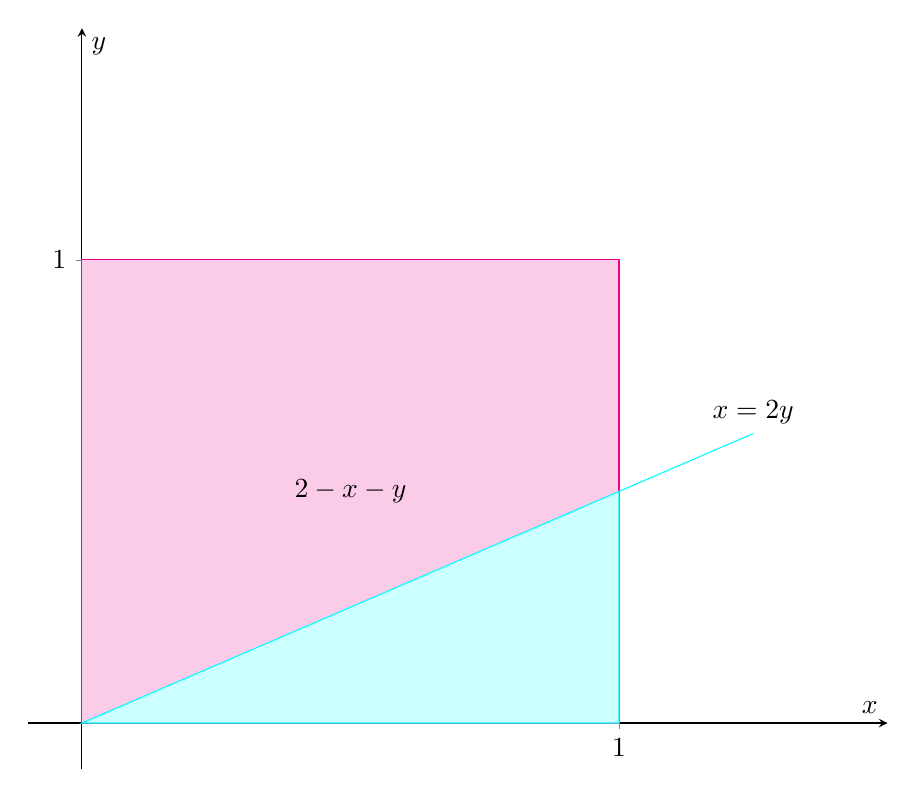
\begin{tikzpicture}
        \begin{axis}[
                axis lines=middle,
                ymin=-0.1,ymax=1.5,
                xmin=-0.1,xmax=1.5,
                xlabel=$x$,
                ylabel=$y$,
                xtick={1},
                ytick={1},
                scale only axis,
                width=0.9\textwidth
            ]
            \draw[color=magenta,fill=magenta!20!white] (axis cs:1,0) -- (axis cs:1,1) -- (axis cs:0,1) -- (axis cs:0,0) -- cycle;
            \node at (axis cs:0.5,0.5) {$2-x-y$};
            \draw[color=Cyan,fill=Cyan!20!white] (axis cs:0,0) -- (axis cs:1,0) -- (axis cs:1,0.5) -- cycle;
            \draw[color=Cyan] (axis cs:1,0.5) -- (axis cs:1.25,0.625) node [color=black,above] {$x=2y$};
        \end{axis}
    \end{tikzpicture}
\end{marginfigure}
\begin{solution}

    \begin{enumerate}[(1)]
        \item 如图,填充部分为概率密度函数$2-x-y$,其余为$0$,而蓝色填充属于$X>2Y$概率不为$0$的区域。
              \[
                  P\{X>2Y\} = \iint\limits_{x>2y} f(x,y) \dd{x}\dd{y}
                  = \int_0^1\dd{x}\int_0^{x/2} 2-x-y\dd{y}
                  = \frac{7}{24}
              \]
        \item \[ F_Z(z) = P\{Z\leq z\} = P\{X+Y\leq z\} \]
              \begin{center}
                  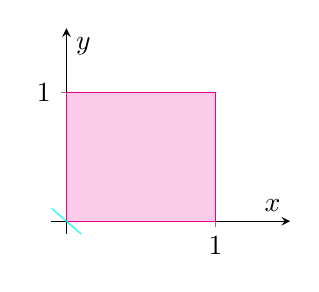
\begin{tikzpicture}
                      \begin{axis}[
                              axis lines=middle,
                              ymin=-0.1,ymax=1.5,
                              xmin=-0.1,xmax=1.5,
                              xlabel=$x$,
                              ylabel=$y$,
                              xtick={1},
                              ytick={1},
                              scale only axis,
                              width=0.25\textwidth
                          ]
                          \draw[color=magenta,fill=magenta!20!white] (axis cs:1,0) -- (axis cs:1,1) -- (axis cs:0,1) -- (axis cs:0,0) -- cycle;
                          \draw[color=Cyan] (axis cs:0.1,-0.1) -- (axis cs:-0.1,0.1);
                      \end{axis}
                  \end{tikzpicture}
                  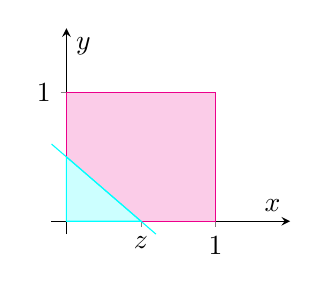
\begin{tikzpicture}
                      \begin{axis}[
                              axis lines=middle,
                              ymin=-0.1,ymax=1.5,
                              xmin=-0.1,xmax=1.5,
                              xlabel=$x$,
                              ylabel=$y$,
                              xtick={1,0.5},
                              ytick={1},
                              xticklabels={1,$z$},
                              scale only axis,
                              width=0.25\textwidth
                          ]
                          \draw[color=magenta,fill=magenta!20!white] (axis cs:1,0) -- (axis cs:1,1) -- (axis cs:0,1) -- (axis cs:0,0) -- cycle;
                          \draw[color=Cyan,fill=Cyan!20!white] (axis cs:0.5,0) -- (axis cs:0,0.5) -- (axis cs:0,0) -- cycle;
                          \draw[color=Cyan] (axis cs:0.6,-0.1) -- (axis cs:-0.1,0.6);
                      \end{axis}
                  \end{tikzpicture}
                  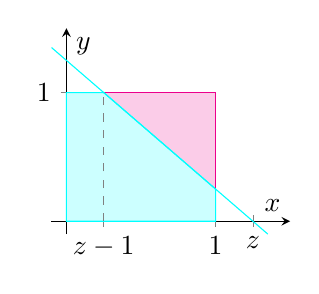
\begin{tikzpicture}
                      \begin{axis}[
                              axis lines=middle,
                              ymin=-0.1,ymax=1.5,
                              xmin=-0.1,xmax=1.5,
                              xlabel=$x$,
                              ylabel=$y$,
                              xtick={1,0.25,1.25},
                              ytick={1},
                              xticklabels={1,$z-1$,$z$},
                              scale only axis,
                              width=0.25\textwidth
                          ]
                          \draw[color=magenta,fill=magenta!20!white] (axis cs:1,0) -- (axis cs:1,1) -- (axis cs:0,1) -- (axis cs:0,0) -- cycle;
                          \draw[color=Cyan,fill=Cyan!20!white] (axis cs:0,0) -- (axis cs:1,0) -- (axis cs:1,0.25) -- (axis cs:0.25,1) -- (axis cs:0,1) -- cycle;
                          \draw[color=Cyan] (axis cs:1.35,-0.1) -- (axis cs:-0.1,1.35);
                          \draw[Gray,dashed] (axis cs:0.25,0) -- (axis cs:0.25,1);
                      \end{axis}
                  \end{tikzpicture}
              \end{center}
              根据上图可以得知

              当$z\leq 0$时,必有$F_Z(z)=0$;

              当$z\geq 2$时,$F_Z(z)=1$;

              下面考虑$0<z<2$的情况,

              当$0<z<1$时,$0<y\leq z-x$,则有
              \[ F_Z(z) = \int_0^z\dd{x}\int_0^{z-x} 2-x-y\dd{y} = -\frac{1}{3}z^3 + z^2 \]

              当$1\leq z < 2$时,则为整个区域减去右上的小三角积分
              \[ F_Z(z) = 1 - \int_{z-1}^1\dd{x}\int_{z-x}^1 2-x-y\dd{y}= \frac{1}{3}z^3 -2z^2+4z -\frac{5}{3} \]

              综上所述,
              \[
                  F_Z(z) =
                  \begin{dcases}
                      0,                                    & z\leq 0,   \\
                      -\frac{1}{3}z^3+z^2,                  & 0<z\leq 1, \\
                      \frac{1}{3}z^3 -2z^2+4z -\frac{5}{3}, & 1<z < 2,   \\
                      1,                                    & 2\leq z.
                  \end{dcases}
              \]
              因此
              \[
                  f_Z(z) = F_Z'(z) =
                  \begin{cases}
                      -z^2+2z,  & 0<z\leq 1,   \\
                      z^2-4z+4, & 1<z<2,       \\
                      0,        & \text{其它}.
                  \end{cases}
              \]
    \end{enumerate}
\end{solution}

\section{数字特征}
\subsection{数学期望}
离散型随机变量的数学期望为
\begin{equation}
    E(X) = \sum_{i=1}^\infty x_ip_i
\end{equation}
且级数绝对收敛。

连续型随机变量$X\sim f(x)$的数学期望为
\begin{equation}
    E(X) = \int_{-\infty}^{+\infty} xf(x)\dd{x}
\end{equation}
且无穷积分绝对收敛。

\begin{example}
    3双不同的鞋,逐个抽取,平均抽几次才能凑出一双。
\end{example}
\begin{solution}
    设抽$X$次,则$X=2,3,4$,那么有
    \begin{align*}
        P(X=2) & = \frac{C_6^1C_1^1}{A_6^2} = \frac{1}{5}            \\
        P(X=4) & = \frac{C_6^1C_4^1C_2^1 C_3^1}{A_6^4} = \frac{2}{5} \\
        P(X=3) & = 1-P(X=2)-P(X-4) = \frac{2}{5}
    \end{align*}
    则
    \[ E(X) = 2\times \frac{1}{5} + 3 \times \frac{2}{5} + 4\times \frac{2}{5} = \frac{16}{5} \]
\end{solution}

期望的性质
\begin{enumerate}[(1)]
    \item $E(C)=c$,即常数的期望也为常数;
    \item $E(cX) = cE(X)$;
    \item $E(X\pm Y)=E(X)\pm E(Y)$;
    \item $E(XY)=E(X)E(Y)$,其中$X,Y$不相关。
\end{enumerate}

\begin{example}
    已知
    \[
        X \sim f(x) =
        \begin{dcases}
            \frac{x^n}{n!}\mathrm{e}^{-x}, & x>0,     \\
            0,                             & x\leq 0.
        \end{dcases}
    \]
    求$E(X)$
\end{example}
\begin{solution}
    \[
        E(X) = \int_{-\infty}^{+\infty} xf(x)\dd{x}
        =\int_0^{+\infty} \frac{x^{n+1}}{n!}\mathrm{e}^{-x}\dd{x}
        =\frac{1}{n!}\int_0^{+\infty} x^{n+1}\mathrm{e}^{-x}\dd{x}
        =\frac{\Gamma(n+2)}{n!} = n+1
    \]
\end{solution}

\subsubsection{函数的期望}
若$Y=g(X)$,$X$为离散型随机变量,则有
\begin{equation}
    E(Y)=E[g(X)] = \sum_{i} g(x_i)p_i
\end{equation}
且级数绝对收敛。

若$Y=g(X)$,$X$为连续型随机变量,则有
\begin{equation}
    E(Y)=E[g(X)] = \int_{-\infty}^{+\infty} g(x)f(x)\dd{x}
\end{equation}
且无穷积分绝对收敛。

若$Z=g(X,Y)$,且$(X,Y)\sim P\{X=x_i,Y=y_j\}=p_{ij},\  i,j=1,2,3,\cdots$
则有
\begin{equation}
    E(Z) = E[g(X,Y)] = \sum_i \sum_j g(x_i,y_j)p_{ij}
\end{equation}
且级数绝对收敛。

若$Z=g(X,Y)$,且$(X,Y)\sim f(x,y)$,则有
\begin{equation}
    E(Z) = E[g(X,Y)] = \int_{-\infty}^{+\infty} \int_{-\infty}^{+\infty} g(x,y)f(x,y)\dd{x}\dd{y}
\end{equation}

\subsection{方差}
.
\begin{definition}
    在概率论和统计学中,一个随机变量的方差描述的是它的离散程度,也就是该变量离其期望值的\textcolor{red}{距离}。
    \[ D(X) = E\left[(X-E(X))^2\right] \]
    显然方差非负。
\end{definition}
将定义式展开
\begin{align*}
    D(X) & = E\left[X^2 -2XE(X)+(E(X))^2\right] \\
         & = E(X^2)-2E(X)E(E(X))+[E(X)]^2       \\
         & = E(X^2)- 2[E(X)]^2 + [E(X)]^2       \\
         & = E(X^2) - [E(X)]^2
\end{align*}
即有如下关系式
\begin{equation}
    D(X) = E(X^2) - [E(X)]^2
\end{equation}
由于方差非负,对上式移向可得不等式
\begin{equation}
    E(X^2)\geq [E(X)]^2
\end{equation}

方差有如下性质
\begin{enumerate}[(1)]
    \item $D(C)=0$,即常数的方差为零;
    \item $D(aX+b) = a^2D(X)$;
    \item $D(X\pm Y) = D(X)+D(Y)$,其中$X,Y$不相关。
    \item $D(aX+bY)=a^2D(X)+b^2D(Y) + 2ab\operatorname{Cov}(X,Y)$
\end{enumerate}

\subsection{协方差,相关系数}
协方差(Covariance)用于衡量两个随机变量的联合变化程度。而方差是协方差的一种特殊情况,即变量与自身的协方差。
\begin{definition}
    随机变量$X$与$Y$之间的协方差定义为
    \[ \operatorname{Cov}(X,Y) = E[(X-E(X))(Y-E(Y))] \]
\end{definition}
将协方差的定义式展开,即
\begin{align*}
    \operatorname{Cov}(X,Y) & = E[XY -XE(Y) - YE(X) + E(X)E(Y)]     \\
                            & =E(XY) -E[XE(Y)] - E[YE(X)] +E(X)E(Y) \\
                            & =E(XY) - E(X)E(Y)
\end{align*}
所以有如下等式
\begin{equation}
    \operatorname{Cov}(X,Y) = E(XY)-E(X)E(Y)
\end{equation}
因此,当$X,Y$不相关时,$\operatorname{Cov}(X,Y)=0$

协方差有如下性质
\begin{enumerate}[(1)]
    \item $\operatorname{Cov}(X,C)=0$,其中$C$为常数;
    \item $\operatorname{Cov}(X,Y) = \operatorname{Cov}(Y,X)$;
    \item $\operatorname{Cov}(aX,bY)=ab\operatorname{Cov}(X,Y)$;
    \item $\operatorname{Cov}(X_1+X_2,Y)=\operatorname{Cov}(X_1,Y)+\operatorname{Cov}(X_2,Y)$;
    \item $D(X\pm Y) = D(X)+D(Y)\pm 2\operatorname{Cov}(X,Y)$。
\end{enumerate}

\begin{example}
    已知$X_1,X_2,\cdots,X_n$独立,且均服从$N(0,\sigma^2)$,求$\operatorname{Cov}\left(X_1, \frac{1}{n}\sum_{i=1}^n X_i\right)$
\end{example}
\begin{solution}
    \[
        \operatorname{Cov}\left(X_1, \frac{1}{n}\sum_{i=1}^n X_i\right)
        =
        \operatorname{Cov}\left(X_1,\frac{1}{n}X_1\right) + \cdots + \operatorname{Cov}\left(X_1,\frac{1}{n}X_n\right)
        =
        \frac{1}{n}\operatorname{Cov}(X_1,X_1) + 0
        =
        \frac{\sigma^2}{n}
    \]
\end{solution}

\begin{example}
    现有1个红球,2个白球,3个黑球,从中任取2个,其中$X$个红球,$Y$个白球,求
    \begin{enumerate}[(1)]
        \item $(X,Y)$的分布;
        \item $\operatorname{Cov}(X,Y)$。
    \end{enumerate}
\end{example}
\begin{solution}
    \begin{align*}
        P(X=0,Y=0) & = \frac{C_3^2}{C_6^2} = \frac{1}{5}       \\
        P(X=0,Y=1) & = \frac{C_2^1C_3^1}{C_6^2} = \frac{2}{5}  \\
        P(X=0,Y=2) & = \frac{C_2^2}{C_6^2} = \frac{1}{15}      \\
        P(X=1,Y=0) & = \frac{C_1^1C_3^1}{C_6^2} = \frac{1}{5}  \\
        P(X=1,Y=1) & = \frac{C_1^1C_2^1}{C_6^2} = \frac{2}{15} \\
        P(X=1,Y=2) & = 0
    \end{align*}
    因此$(X,Y)$的分布律为
    \[
        \begin{array}{c|ccc}
            X\backslash Y & 0            & 1             & 2             \\ \hline
            0             & \dfrac{1}{5} & \dfrac{2}{5}  & \dfrac{1}{15} \\ [2ex]
            1             & \dfrac{1}{5} & \dfrac{2}{15} & 0
        \end{array}
    \]
    因此
    \begin{align*}
        P(XY=0) & = \frac{1}{5}+\frac{2}{15}+\frac{1}{15}+\frac{1}{5}= \frac{13}{15} \\
        P(XY=1) & =\frac{2}{15}                                                      \\
        P(XY=2) & =0
    \end{align*}
    则
    \begin{align*}
        E(XY) & =\frac{2}{15}                                          \\
        E(X)  & =\frac{1}{5}+\frac{2}{15}=\frac{1}{3}                  \\
        E(Y)  & = \frac{2}{5}+\frac{2}{15}+2\frac{1}{15} = \frac{2}{3}
    \end{align*}
    \[ \operatorname{Cov}(X,Y) = E(XY) - E(X)E(Y) = -\frac{4}{45} \]
\end{solution}

\begin{definition}
    $X,Y$的相关系数定义为
    \[
        \rho_{XY} =
        \begin{dcases}
            \frac{\operatorname{Cov}(X,Y)}{\sqrt{D(X)}\sqrt{D(Y)}}, & D(X)D(Y)\neq 0 \\
            0,                                                      & D(X)D(Y)=0
        \end{dcases}
    \]
    当$\rho_{XY}=0$时,则称$X,Y$不相关。
\end{definition}
需要注意的是:
\begin{enumerate}
    \item \textcolor{red}{独立一定不相关,不相关不一定独立};
    \item \textcolor{red}{若$(X,Y)$服从正态分布,则有$X,Y\text{独立}\iff \rho = 0$,逆反命题$X,Y\text{不独立}\iff \rho \neq 0$}
\end{enumerate}

相关系数的性质如下
\begin{enumerate}[(1)]
    \item $\abs{\rho_{XY}}\leq 1$;
    \item $\abs{\rho_{XY}}=1 \iff P\{Y=aX+b\},a\neq 0$
\end{enumerate}
\begin{example}
    某试验有三种概率均为$\frac{1}{3}$的两两不先关的结果$A_1,A_2,A_3$,将试验独立重复$2$次,
    $X$表示$2$次实验中$A_1$发生的次数,$Y$表示$2$次实验中$A_2$发生的次数,求$X,Y$的相关系数。
\end{example}
\begin{solution}
    根据题意$X$和$Y$都服从二项分布$B(2,\frac{1}{3})$,设两次试验中$A_3$发生的次数为$Z$。
    则有$X+Y+Z=2$,故而有
    \begin{align*}
        \operatorname{Cov}(X,Y) & = \operatorname{Cov}(X,2-X-Z)                                              \\
                                & = \operatorname{Cov}(X,2)-\operatorname{Cov}(X,X) -\operatorname{Cov}(X,Z) \\
                                & =-D(X) - \operatorname{Cov}(X,Y) \qquad\text{(对称性)}
    \end{align*}
    所以$\operatorname{Cov}(X,Y)= -\frac{D(X)}{2}$,又$D(X)=D(Y)$
    则相关系数为
    \[ \rho_{XY} = \frac{\operatorname{Cov}(X,Y)}{\sqrt{D(X)}\sqrt{D(Y)}} = \frac{-D(X)/2}{D(X)}=-\frac{1}{2} \]
\end{solution}

\section{大数定理,中心极限定理}
\paragraph{切比雪夫不等式}:
\begin{align}
    \label{eq:切比雪夫不等式}
    P\{\abs{X-E(X)}\geq \varepsilon\} & \leq \frac{D(X)}{\varepsilon^2} \qquad    & (\varepsilon > 0) \\
    P\{\abs{X-E(X)} < \varepsilon \}  & \geq 1- \frac{D(X)}{\varepsilon^2} \qquad & (\varepsilon > 0)
\end{align}

\begin{example}
    \[
        X\sim f(x) =
        \begin{cases}
            2\mathrm{e}^{-2x}, & x>0,     \\
            0,                 & x\leq 0.
        \end{cases}
    \]
    \begin{enumerate}[(1)]
        \item 根据切比雪夫不等式估计$P\{X\geq\frac{3}{2}\} \leq A$;
        \item 直接计算$P\{X\geq \frac{3}{2}\}$
    \end{enumerate}
\end{example}
\begin{solution}
    \begin{enumerate}[(1)]
        \item 显然$X\sim E(2)$,所以有$E(X) = \frac{1}{\lambda} = \frac{1}{2}, D(X)=\frac{1}{\lambda^2}=\frac{1}{4}$
              \begin{align*}
                  P\left\{X\geq \frac{3}{2}\right\} & = P\left\{ X - \frac{1}{2} \geq 1 \right\} = P\left\{ \abs{X-\frac{1}{2}} \geq 1 \right\} - P\left\{X-\frac{1}{2} \leq -1\right\}   \\
                                                    & =P\left\{ \abs{X-\frac{1}{2}} \geq 1 \right\} - P\left\{ X\leq -\frac{1}{2} \right\} = P\left\{ \abs{X-\frac{1}{2}} \geq 1 \right\} \\
                                                    & \leq \frac{D(X)}{1^2} = \frac{1}{4}
              \end{align*}
              即
              \[ P\left\{X\geq \frac{3}{2}\right\} \leq \frac{1}{4} \]
        \item \[ P\left\{ X\geq \frac{3}{2} \right\} = \mathrm{e}^{-2\times \frac{3}{2}} = \mathrm{e}^{-3} \]
    \end{enumerate}
\end{solution}

\begin{example}
    已知$X\sim f(x), D(X) = 1, Y\sim f(-y)$,且$X,Y$的相关系数为$-\frac{1}{4}$,利用切比雪夫不等式估计
    $P\{\abs{X+Y}\geq 2\} \leq A$
\end{example}
\begin{solution}
    令$Z=X+Y$,则
    \begin{align*}
        E(Z) & = E(X+Y) = E(X) + E(Y)                            \\
             & = E(X) + \int_{-\infty}^{+\infty} yf(-y)\dd{y}    \\
             & = E(X) + \int_{+\infty}^{-\infty} (-m)f(m)\dd{-m} \\
             & =E(X) - E(X)                                      \\
             & = 0
    \end{align*}
    由上述过程可知$E(X)=-E(Y)$,所以
    \begin{align*}
        D(Y) & = E(Y^2)+[E(Y)]^2 = \int_{-\infty}^{+\infty} y^2f(-y)\dd{y} + [E(X)]^2 \\
             & =\int_{+\infty}^{-\infty} (-m)^2f(m)\dd(-m)+ [E(X)]^2                  \\
             & =E(X^2)+[E(X)]^2                                                       \\
             & =D(X)
    \end{align*}
    因此
    \begin{align*}
        D(Z) & = D(X+Y) = D(X)+D(Y) +2\operatorname{Cov}(X,Y) \\
             & = 2D(X)+ 2\rho_{XY}\sqrt{D(X)}\sqrt{D(Y)}      \\
             & = 2D(X) + 2\times\left(-\frac{1}{4}\right)D(X) \\
             & = \frac{3}{2}
    \end{align*}
    \[ P\{\abs{X+Y}\geq 2\}  = P\{ \abs{Z-E(X)}\geq 2 \} \leq \frac{D(Z)}{2^2}=\frac{3}{8} \]
\end{solution}

\begin{definition}
    (依概率收敛)
    设$X_1,X_2,\cdots,X_n,\cdots$为随机变量序列,$A$为常数,$\forall \varepsilon >0$,若有
    \[ \lim_{n\to \infty} P\{\abs{X_n - A} < \varepsilon \} = 1  \]
    则称随机变量序列的依概率收敛于$A$,记作$X_n \xrightarrow{p} A$
\end{definition}

\paragraph{切比雪夫大数定理}
设$X_1,X_2,\cdots,X_n,\cdots$两两不相关,且方差有界,则$\forall \varepsilon >0$
\begin{equation}
    \label{eq:切比雪夫大数定理}
    \lim_{n\to\infty} P\left\{ \abs{\frac{1}{n}\sum_{i=1}^n X_i - \frac{1}{n}\sum_{i=1}^n E(X_i)} < \varepsilon \right\} = 1
\end{equation}

\paragraph{辛钦大数定理}
设$X_1,X_2,\cdots,X_n,\cdots$独立同分布,且$E(X_i)=\mu$,则$\forall \varepsilon > 0$
\begin{eqnarray}
    \label{eq:辛钦定理}
    \lim_{n\to \infty} P\left\{ \abs{\frac{1}{n}\sum_{i=1}^n X_i - \mu} < \varepsilon \right\} = 1
\end{eqnarray}

\paragraph{伯努利大数定理}
$X_n \sim B(n,p)$,则$\forall \varepsilon > 0$,都有
\begin{equation}
    \label{eq:伯努利大数定理}
    \lim_{n\to \infty} P\left\{ \abs{\frac{X_n}{n} - p} < \varepsilon \right\} = 1
\end{equation}
这是辛钦大数定律的特例,因为$X_n = Y_1+Y_2+\cdots+Y_n$,且$Y_i\sim B(1,p)$,所以将其带入辛钦大数定理可得出伯努利大数定理。

\paragraph{中心极限定理}
设随机变量$X_1,X_2,\cdots,X_n$独立同分布,且具有有限的数学期望$\mu$和方差$\sigma^2$,则有
\begin{equation}
    \label{eq:中心极限定理}
    \lim_{n\to\infty} P\left\{ \frac{\sum_{i=1}^n X_i - n\mu}{\sqrt{n}\sigma} \leq x \right\} = \Phi(x)
\end{equation}

这里可以理解为,当$X_1,X_2,\cdots$足够多时,对新的变量$\sum X_i$进行标准化,其近似服从标准正态分布,这里标准化需要的参数如下
\begin{align*}
    E\left(\sum_{i=1}^n X_i\right) & = n\mu      \\
    D\left(\sum_{i=1}^n X_i\right) & = n\sigma^2
\end{align*}

\begin{example}
    设$X_1,X_2,\cdots,X_n,\cdots$独立同分布$B(1,\frac{1}{2})$,则
    \begin{tasks}[label=(\Alph*),label-width = 2em](2)
        \task $\displaystyle \lim_{n\to\infty} P\left\{ \frac{\sum_{i=1}^n X_i - 2n}{2\sqrt{n}} \leq x \right\}=\Phi(x)$
        \task $\displaystyle \lim_{n\to\infty} P\left\{ \frac{\sum_{i=1}^n X_i - 2n}{\sqrt{2n}} \leq x \right\}=\Phi(x)$
        \task $\displaystyle \lim_{n\to\infty} P\left\{ \frac{2\sum_{i=1}^n X_i - n}{\sqrt{n}} \leq x \right\}=\Phi(x)$
        \task $\displaystyle \lim_{n\to\infty} P\left\{ \frac{\sum_{i=1}^n X_i - n}{\sqrt{n}} \leq x \right\}=\Phi(x)$
    \end{tasks}
\end{example}
\begin{solution}
    根据选项的形式,考虑中心极限定理,则有$\mu = \frac{1}{2}, \sigma^2 = \frac{1}{4}$,则
    \[
        \lim_{n\to\infty} P\left\{ \frac{\sum_{i=1}^n X_i - \frac{1}{2}n}{\frac{1}{2}\sqrt{n}} \right\}
        = \lim_{n\to\infty} P\left\{ \frac{2\sum_{i=1}^n X_i - n}{\sqrt{n}} \leq x \right\}=\Phi(x)
    \]
    选(C)
\end{solution}

当题目出现多个随机变量的概率时,如果有$\lim_{n\to\infty}$,那么就要考虑中心极限定理,而大数定理则是考虑依概率收敛问题,其极限值为$1$,
若没有$\lim_{n\to\infty}$,那么就要考虑切比雪夫不等式。

\section{数理统计基本概念}
\subsection{总体、样本、统计量、数字特征}
\textcolor{red}{相互独立}且与总体$X$\textcolor{red}{同分布}的随机变量$X_1,X_2,\cdots,X_n$称为简单随机样本,简称\textcolor{red}{样本},
$x_1,x_2,\cdots,x_n$称为样本值或观察值。

因此有$X\sim F(x)$,则样本$X_1,X_2,\cdots,X_n$的联合分布函数为
\begin{equation}
    F_n(x_1,x_2,\cdots,x_n)
    = P\{X_1\leq x_1, X_2\leq x_2,\cdots,X_n\leq x_n\}
    = \prod_{i=1}^n P\{X_i\leq x_i\}
    = \prod_{i=1}^n F(x_i)
\end{equation}

若$X\sim f(x)$,同理有样本$X_1,X_2,\cdots,X_n$的联合密度函数为
\begin{equation}
    f_n(x_1,x_2,\cdot,x_n) = \prod_{i=1}^n f(x_i)
\end{equation}

\begin{example}
    若$X\sim N(\mu,\sigma^2),\sigma>0$,样本$X_1,X_2,\cdots,X_n$的联合密度函数为?
\end{example}
\begin{solution}
    \begin{align*}
        f(x_1,x_2,\cdots,x_n)
         & = \prod_{i=1}^n \frac{1}{\sigma\sqrt{2\pi}}\exp{-\frac{(x_i-\mu)^2}{2\sigma^2}}                \\
         & = \left(\frac{1}{\sigma\sqrt{2\pi}}\right)^n \exp{-\frac{\sum_{i=1}^n (x_i-\mu)^2}{2\sigma^2}}
    \end{align*}
\end{solution}

\begin{example}
    若$X\sim P(\lambda)$,样本$X_1,X_2,\cdots,X_n$的联合概率为
\end{example}
\begin{solution}
    \begin{align*}
        P\{X_1=x_1,X_2=x_2,\cdots,X_n=x_n\}
         & = \prod_{i=1}^n P\{X_i=x_i\}                                                   \\
         & = \prod_{i=1}^n \frac{\lambda^{x_i}}{x_i!}\mathrm{e}^{-\lambda}                \\
         & = \frac{\lambda^{\sum_{i=1}^n x_i}}{\prod_{i=1}^n x_i!} \mathrm{e}^{-n\lambda}
    \end{align*}
\end{solution}

样本$X_1,X_2,\cdots,X_n$的不含未知参数的函数$T=T(X_1,X_2,\cdots,X_n)$称为样本的\textcolor{red}{\textbf{\textsf{统计量}}},
如果$x_1,x_2,\cdots,x_n$是样本$X_1,X_2,\cdots,X_n$的观察值,则$T(x_1,x_2,\cdots,x_n)$是统计量$T(X_1,X_2,\cdots,X_n)$的观察值。

一些统计量如下
\begin{enumerate}[(1)]
    \item 样本均值$\displaystyle \bar{X}=\frac{1}{n}\sum_{i=1}^n X_i$;
    \item 样本方差$\displaystyle s^2 = \frac{1}{n-1}\sum_{i=1}^n \left(X_i - \bar{X}\right)^2$;
    \item 标准差$s = \sqrt{s^2}$;
\end{enumerate}

这些统计量有如下性质:若样本$X_1,X_2,\cdots,X_n$与总体$X$同分布,且$E(X)=\mu, D(X) = \sigma^2$,则有
\begin{enumerate}[(1)]
    \item $E\left(\bar{X}\right) = \frac{1}{n}\sum_{i=1}^n (X_i) = \mu = E(X)$;
    \item $D\left(\bar{X}\right) = \frac{1}{n^2}\sum_{i=1}^n(X_i) = \frac{\sigma^2}{n} = \frac{D(X)}{n}$;
    \item $E(s^2) = \sigma^2 = D(X)$
\end{enumerate}

\begin{example}
    设$X\sim B(1,p)$,求样本$X_1,X_2,\cdots,X_n$的统计量$\bar{X}$的分布。
\end{example}
\begin{solution}
    如果用定义法做,那么会有$n$重积分,显然非常困难。由于$X\sim B(1,p)$,且样本的随机变量相互独立,那么显然
    $\displaystyle \sum_{i=1}^n X_i \sim B(n,p)$,因此就有
    \[ P\left\{ \sum_{i=1}^n X_i = k \right\} = C_n^kp^k(1-p)^{n-k}, \qquad k=0,1,2,\cdots \]
    所以
    \[ P\left\{ \bar{X} = \frac{k}{n} \right\} = C_n^kp^k(1-p)^{n-k}, \qquad k=0,1,2,\cdots \]
    注意$\bar{X}$的分布并不是二项分布,因为括弧里的等号右侧不是$k$,而是$k/n$
\end{solution}

\begin{example}
    设$\displaystyle X\sim f(x) = \frac{1}{2}\mathrm{e}^{-\abs{x}}$,其$X_1,X_2,\cdots,X_n$的样本方差为$s^2$,
    求$E(s^2)$.
\end{example}
\begin{solution}
    \[ E\left(s^2\right)  = D(X) = E\left(X^2\right) - [E(X)]^2 \]
    \begin{align*}
        E(X)              & = \int_{-\infty}^{+\infty}\frac{1}{2}x\mathrm{e}^{-\abs{x}}\dd{x} = 0 \\
        E\left(X^2\right) & = \int_{-\infty}^{+\infty} \frac{1}{2}x^2\mathrm{e}^{-\abs{x}} \dd{x}
        = \int_{0}^{+\infty}x^2\mathrm{e}^{-x}\dd{x} = \Gamma(3) = 2
    \end{align*}
    所以$E\left(s^2\right) = 2$
\end{solution}

\begin{example}
    若$X_1,X_2,\cdots,X_n$为来自总体$X\sim N\left(-1,\sigma^2\right)$的样本,且
    \[
        T_1 = \frac{1}{n}\sum_{i=1}^n X_i, \qquad T_2 = \frac{1}{n-1}\sum_{i=1}^{n-1}X_i + \frac{1}{n}X_n
    \],则
    \begin{tasks}[label=(\Alph*),label-width = 2em](2)
        \task $ET_1 > ET_2,\ DT_1 > DT_2$
        \task $ET_1 > ET_2,\ DT_1 < DT_2$
        \task $ET_1 < ET_2,\ DT_1 > DT_2$
        \task $ET_1 < ET_2,\ DT_1 < DT_2$
    \end{tasks}
\end{example}
\begin{solution}
    \begin{align*}
        ET_1 & = \frac{1}{n}\sum_{i=1}^n EX_i = -\frac{n}{n} = -1                                                                   \\
        ET_2 & = \frac{1}{n-1}\sum_{i=1}^{n-1}EX_i + \frac{1}{n}EX_n = -\left(\frac{n-1}{n-1}+\frac{1}{n}\right) = -1 - \frac{1}{n} \\
        DT_1 & = \frac{1}{n^2}\sum_{i=1}^n DX_i = \frac{1}{n}\sigma^2                                                               \\
        DT_2 & = \frac{1}{(n-1)^2}\sum_{i=1}^{n-1}DX_i + \frac{1}{n^2}DX_n = \left(\frac{1}{n-1}+\frac{1}{n^2}\right)\sigma^2
    \end{align*}
    所以$ET_1>ET_2,\ DT_1<DT_2$,选(B)
\end{solution}


\subsection{常用统计分布}
\subsubsection{\texorpdfstring{$\chi^2$}{χ}分布}
.
\begin{definition}
    若$X_1,X_2,\cdots,X_n$相互独立且均服从标准正态分布$N(0,1)$,则
    \[ X = X_1^2 + X_2^2 + \cdots + X_n^2 \]
    称为$\chi^2$分布,记为$X\sim \chi^2(n)$,其中$n$称为自由度。
\end{definition}
显然满足$\chi^2$分布的随机变量一定大于零。对于卡方分布,有下面这些性质
\begin{enumerate}[(1)]
    \item $E\left(\chi^2(n)\right) = n$;
    \item $D\left(\chi^2(n)\right) = 2n$;
    \item 若$\chi_1^2(n_1), \chi_2^2(n_2)$独立,则$\chi_1^2(n_1) + \chi_2^2(n_2) \sim \chi^2(n_1+n_2)$
\end{enumerate}

\begin{example}
    样本$X_1,X_2,X_3$来自总体$N(0,4)$,已知$X=a(X_1-2X_2+3X_3)^2\sim \chi^2$,求$a$
\end{example}
\begin{solution}
    由于$X\sim \chi^2$,那么显然自由度$n=1$,因此$\sqrt{X}\sim N(0,1)$,即
    \[ \sqrt{a}(X_1-2X_2+3X_3) \sim N(0,1) \]
    所以
    \begin{align*}
        E(\sqrt{X}) & = \sqrt{a}\left[E(X_1)-2E(X_2)+3E(X_3)\right] = 0 \\
        D(\sqrt{X}) & = a\left[D(X_1)+4D(X_2)+9D(X_3)\right] = 56a = 1
    \end{align*}
    所以$a=\frac{1}{56}$
\end{solution}

\subsubsection{\texorpdfstring{$t$}{t}-分布}
.
\begin{definition}
    若$X\sim N(0,1), Y\sim\chi^2(n)$,且$X,Y$独立,则称
    \[ T = \frac{X}{\sqrt{Y/n}} \]
    服从$t$分布,记为$T\sim t(n)$,其中$n$为自由度。
\end{definition}
$t$分布的性质
\begin{enumerate}[(1)]
    \item 概率密度函数是偶函数,形状类似于标准正态;
\end{enumerate}

\subsubsection{\texorpdfstring{$F$}{F}-分布}
.
\begin{definition}
    若$X\sim \chi^2(n_1), Y\sim\chi^2(n_2)$,且$X,Y$相互独立,则
    \[ F=\frac{X/n_1}{Y/n_2} \]
    服从$F$分布,记为$F\sim F(n_1,n_2)$。
\end{definition}
$F$分布有如下性质
\begin{enumerate}[(1)]
    \item 若$F\sim F(n_1,n_2)$,则$\frac{1}{F} \sim F(n_2,n_1)$
\end{enumerate}


\begin{example}
    $X_1,X_2,X_3,X_4$来自总体$N(1,\sigma^2)$的样本,则$\dfrac{X_1-X_2}{\abs{X_3+X_4-2}}$的分布为
    \begin{tasks}[label=(\Alph*),label-width = 2em](2)
        \task $N(0,1)$
        \task $t(1)$
        \task $\chi^2(1)$
        \task $F(1,1)$
    \end{tasks}
\end{example}
\begin{solution}
    因为$X_1,X_2$为相互独立的正态分布,所以$X_1-X_2$也为正态分布,且$X_1-X_2 \sim N(0,2\sigma^2)$

    同理$X_3+X_4-2 = (X_3-1) + (X_4-1) \sim N(0,2\sigma^2)$,
    那么有
    \begin{align*}
        Y = \frac{X_1-X_2}{\sqrt{2}\sigma}          & \sim N(0,1) \\
        Z =\frac{(X_3-1) + (X_4-1)}{\sqrt{2}\sigma} & \sim N(0,1)
    \end{align*}
    $Y,Z$独立,且$Z^2 \sim \chi^2(1)$,那么
    \[ \frac{X_1-X_2}{\abs{X_3+X_4-2}} = \frac{Y}{\abs{Z}} = \frac{Y}{\sqrt{Z^2/1}} \sim t(1) \]
    选(B)
\end{solution}

\begin{example}
    已知$X\sim t(n), Y\sim F(1,n)$,给定$\alpha, (0<\alpha<0.5)$,常数$c$,且$P\{X>c\}=\alpha$,则$P\left\{Y>c^2\right\}=$
    \begin{tasks}[label=(\Alph*),label-width = 2em](4)
        \task $\alpha$
        \task $1-\alpha$
        \task $2\alpha$
        \task $1-2\alpha$
    \end{tasks}
\end{example}
\begin{solution}
    由于$X\sim t(n)$,所以$X^2 \sim F(1,n)$,即$X^2$和$Y$同分���,因此
    \[ P\left\{ Y > c^2 \right\} = P\left\{ X^2 > c^2 \right\} = P\{ X>c \}+P\{X < -c\} = 2P\{X>c\} = 2\alpha \]
    选(C)

    值得注意的是$\sqrt{Y} \not\sim t(n)$,则是因为$t(n)$的分子是标准正态分布,而$\sqrt{Y}$的分子只有标准正态分布的左半侧(无法取小于$0$部分)
\end{solution}

\subsection{正态总体分布}
若$X\sim N(\mu,\sigma^2)$,则样本$X_1,X_2,\cdots,X_n$的统计量有如下性质
\begin{enumerate}[(1)]
    \item $\bar{X} \sim N\left(\mu,\frac{\sigma^2}{n}\right)$;
    \item $\bar{X}$与$s^2$独立;
    \item $\dfrac{(n-1)s^2}{\sigma^2}\sim \chi^2(n-1)$;
    \item $\dfrac{\bar{X}-\mu}{s/\sqrt{n}}\sim t(n-1)$
\end{enumerate}

\section{参数估计}
\subsection{点估计}
用函数$\hat{\theta}(X_1,X_2,\cdots,X_n)$来估计未知参数$\theta$,\textcolor{red}{估计值}为$\hat{\theta}(x_1,x_2,\cdots,x_n)$,
即点估计。称$\hat{\theta}$是$\theta$的\textcolor{red}{估计量},如果$E\left(\hat{\theta}\right) = \theta$,则称为是无偏估计。

如果$\hat{\theta_1},\hat{\theta_2}$都是$\theta$的无偏估计,若$D\left(\hat{\theta_1}\right)\leq D\left(\hat{\theta_2}\right)$,则
$\hat{\theta_1}$比$\hat{\theta_2}$\textcolor{red}{更有效}。

如果$\hat{\theta}(X_1,X_2,\cdots,X_n)$是$\theta$的估计,如果$\hat{\theta}$的依概率收敛于$\theta$,则称$\hat{\theta}$是$\theta$的\textcolor{red}{一致估计量}。

\begin{example}
    已知
    \[
        X \sim f(x,\theta) =
        \begin{dcases}
            \frac{2x}{3\theta^2}, & \theta<x<2\theta, \\
            0,                    & \text{其它}.
        \end{dcases}
    \]
    若$X_1,X_2,\cdots,X_n$为来自总体$X$的样本,且$\displaystyle E\left(c\sum_{i=1}^n X_i^2\right)=\theta^2$,求$c$的值。
\end{example}
\begin{solution}
    \begin{align*}
        E\left(c\sum_{i=1}^n X_i^2\right)
         & = c\sum_{i=1}^n E\left(X_i^2\right)
        = cnE\left(X^2\right)                                \\
         & = cn\int_{-\infty}^{+\infty} x^2f(x,\theta)\dd{x}
        = cn\int_{\theta}^{2\theta} \frac{2x^3}{3\theta^2}\dd{x}
        = \frac{5cn}{2}\theta^2
        = \theta^2
    \end{align*}
    因此$c=\frac{2}{5n}$
\end{solution}

\begin{example}
    已知$X\sim P(\lambda)$,$X_1,X_2,\cdots,X_n$为来自总体$X$的样本,样本均值为$\bar{X}$,样本方差为$s^2$,
    若$\bar{X}^2+ks^2$为$\lambda^2$的无偏估计,求$k$的值。
\end{example}
\begin{solution}
    \begin{align*}
        E\left(\bar{X}^2 + ks^2\right)
         & = E\left(\bar{X}^2\right) + kE\left(s^2\right)
        = D\left(\bar{X}\right) + \left[E\left(\bar{X}\right)\right]^2 + kD(X) \\
         & = \frac{1}{n}D(X) + \left[E(X)\right]^2 + kD(X)                     \\
         & =(\frac{1}{n}+k)\lambda + \lambda^2
    \end{align*}
    所以$k=-\frac{1}{n}$
\end{solution}

\subsection{估计量求法和区间估计}
\paragraph{矩估计法} 用样本矩估计相应的总体矩;用样本矩的函数估计总体矩相应的函数。

\paragraph{最大似然估计法}
参数$\theta$的似然函数:
\begin{enumerate}[(1)]
    \item 离散总体,$P\{X=a_i\} = p(a_i,\theta), L(\theta) = L(x_1,x_2,\cdots,x_n,\theta) = \prod_{i=1}^n p(x_i,\theta)$
    \item 连续总体,$X\sim f(x,\theta), L(\theta)=L(x_1,x_2,\cdots,x_n,\theta)=\prod_{i=1}^n f(x_i,\theta)$
\end{enumerate}
令似然函数$L(x_1,x_2,\cdots,x_n,\theta)$达到最大值的参数值$\hat{\theta} = \hat{\theta}(x_1,x_2,\cdots,x_n)$
称为未知参数$\theta$的\textcolor{red}{最大似然估计值}。

\begin{example}
    $X\sim P(\lambda)$,样本$X_1,X_2,\cdots,X_n$,求$\lambda$的矩估计。
\end{example}
\begin{solution}
    用样本矩估计总体矩,所以有$E(X)=\bar{X}$,即$\lambda=\bar{X}$,得$\hat{\lambda} = \bar{X}$
\end{solution}

\begin{example}
    $X\sim N(\mu,\sigma^2)$,其中$\mu,\sigma^2$均为未知矩估计,现有样本$X_1,X_2,\cdots,X_n$
    \begin{enumerate}[(1)]
        \item 求参数的矩估计;
        \item 求参数的最大似然估计量。
    \end{enumerate}
\end{example}
\begin{solution}
    \begin{enumerate}[(1)]
        \item 那么总体矩可由样本矩来估计,即
              \begin{align*}
                  E(X)              & = \bar{X}                       \\
                  E\left(X^2\right) & = \frac{1}{n}\sum_{i=1}^n X_i^2
              \end{align*}
              又$E(X) = \mu, E\left(X^2\right) = D(X)+\left[E(X)\right]^2 = \sigma^2+\mu^2$
              所以有,
              \begin{align*}
                  \mu              & = \bar{X}                       \\
                  \sigma^2 + \mu^2 & = \frac{1}{n}\sum_{i=1}^n X_i^2
              \end{align*}
              解得
              \[
                  \begin{dcases}
                      \hat{\mu} = \bar{X} \\
                      \hat{\sigma}^2 = \frac{1}{n}\sum_{i=1}^n \left(X_i^2 - \bar{X}^2\right) = \frac{1}{n}\sum_{i=1}^n\left(X_i-\bar{X}\right)^2
                  \end{dcases}
              \]
        \item 由于$X\sim N\left(\mu,\sigma^2\right)$,所以密度函数
              \[
                  f(x) = \frac{1}{\sigma\sqrt{2\pi}}\mathrm{e}^{-\frac{(x-\mu)^2}{2\sigma^2}}
              \]
              似然函数为
              \[
                  L(x_1,x_2,\cdots,x_n,\mu,\sigma^2) = \prod_{i=1}^n f(x_i) = \left(\frac{1}{\sigma\sqrt{2\pi}}\right)^n\exp{-\frac{\sum_{i=1}^n (x_i-\mu)^2}{2\sigma^2}}
              \]
              两边取对数得
              \[
                  \ln L(\mu,\sigma^2) = -\frac{n}{2} \ln (2\pi) - \frac{n}{2}\ln\left(\sigma^2\right) - \frac{1}{2\sigma^2}\sum_{i=1}^n (x_i-\mu)^2
              \]
              令
              \[
                  \begin{dcases}
                      \pdv{\ln L}{\mu} = \frac{1}{\sigma^2}\sum_{i=1}^n (x_i - \mu) = 0 \\
                      \pdv{\ln L}{\sigma^2} = -\frac{n}{2\sigma^2} + \frac{1}{2\left(\sigma^2\right)^2}\sum_{i=1}^n (x_i-\mu)^2=0
                  \end{dcases}
              \]
              解得\textcolor{red}{最大似然估计值}为
              \[
                  \begin{dcases}
                      \hat{\mu} = \bar{x}, \\
                      \hat{\sigma}^2 = \frac{1}{n}\sum_{i=1}^n \left(x_i-\bar{x}\right)^2
                  \end{dcases}
              \]
              则\textcolor{red}{最大似然估计量}为
              \[
                  \begin{dcases}
                      \hat{\mu} = \bar{X}, \\
                      \hat{\sigma}^2 = \frac{1}{n}\sum_{i=1}^n \left(X_i-\bar{X}\right)^2
                  \end{dcases}
              \]
    \end{enumerate}
\end{solution}

